\documentclass[twoside]{book}

% Packages required by doxygen
\usepackage{fixltx2e}
\usepackage{calc}
\usepackage{doxygen}
\usepackage[export]{adjustbox} % also loads graphicx
\usepackage{graphicx}
\usepackage[utf8]{inputenc}
\usepackage{makeidx}
\usepackage{multicol}
\usepackage{multirow}
\PassOptionsToPackage{warn}{textcomp}
\usepackage{textcomp}
\usepackage[nointegrals]{wasysym}
\usepackage[table]{xcolor}

% Font selection
\usepackage[T1]{fontenc}
\usepackage[scaled=.90]{helvet}
\usepackage{courier}
\usepackage{amssymb}
\usepackage{sectsty}
\renewcommand{\familydefault}{\sfdefault}
\allsectionsfont{%
  \fontseries{bc}\selectfont%
  \color{darkgray}%
}
\renewcommand{\DoxyLabelFont}{%
  \fontseries{bc}\selectfont%
  \color{darkgray}%
}
\newcommand{\+}{\discretionary{\mbox{\scriptsize$\hookleftarrow$}}{}{}}

% Page & text layout
\usepackage{geometry}
\geometry{%
  a4paper,%
  top=2.5cm,%
  bottom=2.5cm,%
  left=2.5cm,%
  right=2.5cm%
}
\tolerance=750
\hfuzz=15pt
\hbadness=750
\setlength{\emergencystretch}{15pt}
\setlength{\parindent}{0cm}
\setlength{\parskip}{3ex plus 2ex minus 2ex}
\makeatletter
\renewcommand{\paragraph}{%
  \@startsection{paragraph}{4}{0ex}{-1.0ex}{1.0ex}{%
    \normalfont\normalsize\bfseries\SS@parafont%
  }%
}
\renewcommand{\subparagraph}{%
  \@startsection{subparagraph}{5}{0ex}{-1.0ex}{1.0ex}{%
    \normalfont\normalsize\bfseries\SS@subparafont%
  }%
}
\makeatother

% Headers & footers
\usepackage{fancyhdr}
\pagestyle{fancyplain}
\fancyhead[LE]{\fancyplain{}{\bfseries\thepage}}
\fancyhead[CE]{\fancyplain{}{}}
\fancyhead[RE]{\fancyplain{}{\bfseries\leftmark}}
\fancyhead[LO]{\fancyplain{}{\bfseries\rightmark}}
\fancyhead[CO]{\fancyplain{}{}}
\fancyhead[RO]{\fancyplain{}{\bfseries\thepage}}
\fancyfoot[LE]{\fancyplain{}{}}
\fancyfoot[CE]{\fancyplain{}{}}
\fancyfoot[RE]{\fancyplain{}{\bfseries\scriptsize Generated by Doxygen }}
\fancyfoot[LO]{\fancyplain{}{\bfseries\scriptsize Generated by Doxygen }}
\fancyfoot[CO]{\fancyplain{}{}}
\fancyfoot[RO]{\fancyplain{}{}}
\renewcommand{\footrulewidth}{0.4pt}
\renewcommand{\chaptermark}[1]{%
  \markboth{#1}{}%
}
\renewcommand{\sectionmark}[1]{%
  \markright{\thesection\ #1}%
}

% Indices & bibliography
\usepackage{natbib}
\usepackage[titles]{tocloft}
\setcounter{tocdepth}{3}
\setcounter{secnumdepth}{5}
\makeindex

% Hyperlinks (required, but should be loaded last)
\usepackage{ifpdf}
\ifpdf
  \usepackage[pdftex,pagebackref=true]{hyperref}
\else
  \usepackage[ps2pdf,pagebackref=true]{hyperref}
\fi
\hypersetup{%
  colorlinks=true,%
  linkcolor=blue,%
  citecolor=blue,%
  unicode%
}

% Custom commands
\newcommand{\clearemptydoublepage}{%
  \newpage{\pagestyle{empty}\cleardoublepage}%
}

\usepackage{caption}
\captionsetup{labelsep=space,justification=centering,font={bf},singlelinecheck=off,skip=4pt,position=top}

%===== C O N T E N T S =====

\begin{document}

% Titlepage & ToC
\hypersetup{pageanchor=false,
             bookmarksnumbered=true,
             pdfencoding=unicode
            }
\pagenumbering{roman}
\begin{titlepage}
\vspace*{7cm}
\begin{center}%
{\Large Multi-\/\+Robot-\/\+System }\\
\vspace*{1cm}
{\large Generated by Doxygen 1.8.11}\\
\end{center}
\end{titlepage}
\clearemptydoublepage
\tableofcontents
\clearemptydoublepage
\pagenumbering{arabic}
\hypersetup{pageanchor=true}

%--- Begin generated contents ---
\chapter{Possible problems}
\label{md_README}
\hypertarget{md_README}{}
Launchfiles for launching the implemented functionalities are given in /multi\+\_\+robot\+\_\+launcher/launch
\begin{DoxyEnumerate}
\item exe\+\_\+demo.\+launch\+: Executes a demo environment within basic funcitonalities of the robot formation can be shown.
\item exe\+\_\+navigation.\+launch\+: Executes an environment within the robot formation can be used in combination with the navigation\+\_\+stack.
\item exe\+\_\+transport.\+launch\+: Executes an environment within the robot formation is carrying a transport object.
\item formation.\+launch\+: This is one of the most important launchfiles for using mobile robot formation. It launchs the robots for the formation and does the nescessary remaping for member parameters.
\item gazebo. launch\+: Just launches the gazeob environment.
\item robot.\+launch\+: This launches the hole robot stuff. Eg. The robot state publisher the localisation node for extended kalman filter and loads parameter for these modules. This file does N\+OT load the Foramtion controller since this is located within the controller package!
\item simulation.\+launch\+: Prepares simulations from skript files (see bash).
\item spawn\+\_\+transport\+\_\+object.\+launch A launch files that is used to spawn generic transport object
\end{DoxyEnumerate}

\section*{How to start a simple formation\+:}


\begin{DoxyEnumerate}
\item Execute exe\+\_\+demo.\+launch {\ttfamily \$roslaunch multi\+\_\+robot\+\_\+launcher exe\+\_\+demo.\+launch}
\item Wait til everything is setup
\item Execute the system handling node {\ttfamily \$rosrun simulation\+\_\+env system\+\_\+handling\+\_\+node -\/plan -\/reference}
\end{DoxyEnumerate}

\section*{How to modifie formation parameters\+:}


\begin{DoxyEnumerate}
\item Goto foramtion.\+yaml in the multi\+\_\+robot\+\_\+launcher package
\item Change the parameter within the file 2a) If you change the number or names of formation memebers make sure that you do the same in the formation.\+launch file in mutli\+\_\+robot\+\_\+launcher package 
\end{DoxyEnumerate}
\chapter{Hierarchical Index}
\section{Class Hierarchy}
This inheritance list is sorted roughly, but not completely, alphabetically\+:\begin{DoxyCompactList}
\item \contentsline{section}{Circle\+Planner\+:\+:Circle\+Plan}{\pageref{structCirclePlanner_1_1CirclePlan}}{}
\item \contentsline{section}{Controller}{\pageref{classController}}{}
\begin{DoxyCompactList}
\item \contentsline{section}{Master}{\pageref{classMaster}}{}
\item \contentsline{section}{Slave}{\pageref{classSlave}}{}
\end{DoxyCompactList}
\item \contentsline{section}{Controller\+:\+:Control\+State}{\pageref{structController_1_1ControlState}}{}
\item \contentsline{section}{Controller\+:\+:Control\+Vector}{\pageref{structController_1_1ControlVector}}{}
\item \contentsline{section}{Laser\+Predictor\+:\+:Data}{\pageref{structLaserPredictor_1_1Data}}{}
\item \contentsline{section}{Formation}{\pageref{classFormation}}{}
\item \contentsline{section}{Formation\+Publisher}{\pageref{classFormationPublisher}}{}
\item \contentsline{section}{Formation\+Subscriber}{\pageref{classFormationSubscriber}}{}
\item \contentsline{section}{Laser\+Predictor\+:\+:Frames}{\pageref{structLaserPredictor_1_1Frames}}{}
\item \contentsline{section}{Laser\+Predictor}{\pageref{classLaserPredictor}}{}
\item \contentsline{section}{Lissajous\+Planner\+:\+:Lissajous\+Plan}{\pageref{structLissajousPlanner_1_1LissajousPlan}}{}
\item \contentsline{section}{Controller\+:\+:Lyapunov\+Parameter}{\pageref{structController_1_1LyapunovParameter}}{}
\item \contentsline{section}{Planner}{\pageref{classPlanner}}{}
\begin{DoxyCompactList}
\item \contentsline{section}{Circle\+Planner}{\pageref{classCirclePlanner}}{}
\item \contentsline{section}{Clicked\+Pose\+Planner}{\pageref{classClickedPosePlanner}}{}
\item \contentsline{section}{Lissajous\+Planner}{\pageref{classLissajousPlanner}}{}
\item \contentsline{section}{Spiralplanner}{\pageref{classSpiralplanner}}{}
\end{DoxyCompactList}
\item \contentsline{section}{Spiralplanner\+:\+:Spiral\+Plan}{\pageref{structSpiralplanner_1_1SpiralPlan}}{}
\item \contentsline{section}{Laser\+Predictor\+:\+:Transforms}{\pageref{structLaserPredictor_1_1Transforms}}{}
\end{DoxyCompactList}

\chapter{Class Index}
\section{Class List}
Here are the classes, structs, unions and interfaces with brief descriptions\+:\begin{DoxyCompactList}
\item\contentsline{section}{\hyperlink{structController_1_1AngleDistanceParameter}{Controller\+::\+Angle\+Distance\+Parameter} \\*Specifies the Parameters of the angle distance based control law }{\pageref{d5/d97/structController_1_1AngleDistanceParameter}}{}
\item\contentsline{section}{\hyperlink{structController_1_1Buffer}{Controller\+::\+Buffer$<$ T $>$} \\*Template for a buffer of a given size and a given type }{\pageref{da/df9/structController_1_1Buffer}}{}
\item\contentsline{section}{\hyperlink{structCirclePlanner_1_1CirclePlan}{Circle\+Planner\+::\+Circle\+Plan} }{\pageref{dc/d44/structCirclePlanner_1_1CirclePlan}}{}
\item\contentsline{section}{\hyperlink{classCirclePlanner}{Circle\+Planner} }{\pageref{dc/d00/classCirclePlanner}}{}
\item\contentsline{section}{\hyperlink{classClickedPosePlanner}{Clicked\+Pose\+Planner} }{\pageref{dc/de5/classClickedPosePlanner}}{}
\item\contentsline{section}{\hyperlink{classController}{Controller} \\*Provides a easy to use implementation of a generic mobile robot controller }{\pageref{d9/d85/classController}}{}
\item\contentsline{section}{\hyperlink{structController_1_1ControlState}{Controller\+::\+Control\+State} \\*Holds the System state combined by the pose of the system, the cartesian velocity and the angular velocity }{\pageref{df/d22/structController_1_1ControlState}}{}
\item\contentsline{section}{\hyperlink{structController_1_1ControlVector}{Controller\+::\+Control\+Vector} \\*A struct that holds linear and angular velocity of the Robot since this are the control variable for kinematic tracking control }{\pageref{da/ddc/structController_1_1ControlVector}}{}
\item\contentsline{section}{\hyperlink{structLaserPredictor_1_1Data}{Laser\+Predictor\+::\+Data} \\*Holds all the data used within the predictor }{\pageref{de/d78/structLaserPredictor_1_1Data}}{}
\item\contentsline{section}{\hyperlink{structgazebo_1_1GazeboRosLinkAttacher_1_1fixedJoint}{gazebo\+::\+Gazebo\+Ros\+Link\+Attacher\+::fixed\+Joint} \\*Internal representation of a fixed joint }{\pageref{d8/d07/structgazebo_1_1GazeboRosLinkAttacher_1_1fixedJoint}}{}
\item\contentsline{section}{\hyperlink{classFormation}{Formation} \\*A Class for handeling basic mobile \hyperlink{structFormation_1_1Robot}{Robot} formation work. Properly adds Robots to a formation and provides basic interpretation tools as the adjacency matrix of the formation }{\pageref{d0/d39/classFormation}}{}
\item\contentsline{section}{\hyperlink{classFormationPublisher}{Formation\+Publisher} }{\pageref{d1/da9/classFormationPublisher}}{}
\item\contentsline{section}{\hyperlink{classFormationSubscriber}{Formation\+Subscriber} }{\pageref{d8/dc8/classFormationSubscriber}}{}
\item\contentsline{section}{\hyperlink{structLaserPredictor_1_1Frames}{Laser\+Predictor\+::\+Frames} \\*Holds the names of all the necessary frames for the prediction class }{\pageref{d1/d8b/structLaserPredictor_1_1Frames}}{}
\item\contentsline{section}{\hyperlink{classgazebo_1_1GazeboRosLinkAttacher}{gazebo\+::\+Gazebo\+Ros\+Link\+Attacher} }{\pageref{dd/d29/classgazebo_1_1GazeboRosLinkAttacher}}{}
\item\contentsline{section}{\hyperlink{classLaserPredictor}{Laser\+Predictor} \\*A class for predictings neighbour robots from the laser scanner data of another robot }{\pageref{d1/dc0/classLaserPredictor}}{}
\item\contentsline{section}{\hyperlink{structLissajousPlanner_1_1LissajousPlan}{Lissajous\+Planner\+::\+Lissajous\+Plan} }{\pageref{d1/d0f/structLissajousPlanner_1_1LissajousPlan}}{}
\item\contentsline{section}{\hyperlink{classLissajousPlanner}{Lissajous\+Planner} }{\pageref{d5/dbf/classLissajousPlanner}}{}
\item\contentsline{section}{\hyperlink{structController_1_1LyapunovParameter}{Controller\+::\+Lyapunov\+Parameter} \\*Specifies the parameters needed for the lyapunov based control law }{\pageref{da/d3d/structController_1_1LyapunovParameter}}{}
\item\contentsline{section}{\hyperlink{classMaster}{Master} \\*Class that implements a master robot for multi robot formation control }{\pageref{d2/dbd/classMaster}}{}
\item\contentsline{section}{\hyperlink{classOdometryPredictor}{Odometry\+Predictor} }{\pageref{d6/d6d/classOdometryPredictor}}{}
\item\contentsline{section}{\hyperlink{classPlanner}{Planner} \\*A generic planner class that provides general interface functions and architecture }{\pageref{da/dfa/classPlanner}}{}
\item\contentsline{section}{\hyperlink{structFormation_1_1Robot}{Formation\+::\+Robot} \\*Holds a robot to handle with formation member stuff }{\pageref{d0/da7/structFormation_1_1Robot}}{}
\item\contentsline{section}{\hyperlink{structFormation_1_1RobotProperties}{Formation\+::\+Robot\+Properties} \\*Defines Properties of a \hyperlink{structFormation_1_1Robot}{Robot} }{\pageref{d3/d81/structFormation_1_1RobotProperties}}{}
\item\contentsline{section}{\hyperlink{classSlave}{Slave} \\*Class that implements a slave robot for multi robot formation control }{\pageref{d8/d18/classSlave}}{}
\item\contentsline{section}{\hyperlink{structSpiralplanner_1_1SpiralPlan}{Spiralplanner\+::\+Spiral\+Plan} }{\pageref{d2/dd8/structSpiralplanner_1_1SpiralPlan}}{}
\item\contentsline{section}{\hyperlink{classSpiralplanner}{Spiralplanner} }{\pageref{d4/dd5/classSpiralplanner}}{}
\item\contentsline{section}{\hyperlink{structStepResposePlanner_1_1StepPlan}{Step\+Respose\+Planner\+::\+Step\+Plan} }{\pageref{d5/d69/structStepResposePlanner_1_1StepPlan}}{}
\item\contentsline{section}{\hyperlink{classStepResposePlanner}{Step\+Respose\+Planner} }{\pageref{d6/d2a/classStepResposePlanner}}{}
\item\contentsline{section}{\hyperlink{structLaserPredictor_1_1Transforms}{Laser\+Predictor\+::\+Transforms} \\*Holds all necessary transformations }{\pageref{d6/d09/structLaserPredictor_1_1Transforms}}{}
\end{DoxyCompactList}

\chapter{Class Documentation}
\hypertarget{structCirclePlanner_1_1CirclePlan}{}\section{Circle\+Planner\+:\+:Circle\+Plan Struct Reference}
\label{structCirclePlanner_1_1CirclePlan}\index{Circle\+Planner\+::\+Circle\+Plan@{Circle\+Planner\+::\+Circle\+Plan}}
\subsection*{Public Attributes}
\begin{DoxyCompactItemize}
\item 
float {\bfseries r}\hypertarget{structCirclePlanner_1_1CirclePlan_a713b4aad1fdffcdc82cc2242a87c9203}{}\label{structCirclePlanner_1_1CirclePlan_a713b4aad1fdffcdc82cc2242a87c9203}

\item 
float {\bfseries omega}\hypertarget{structCirclePlanner_1_1CirclePlan_a3bd3fe64ecc478997f8ffe85be6aaa4e}{}\label{structCirclePlanner_1_1CirclePlan_a3bd3fe64ecc478997f8ffe85be6aaa4e}

\end{DoxyCompactItemize}


The documentation for this struct was generated from the following file\+:\begin{DoxyCompactItemize}
\item 
simulation\+\_\+env/include/simulation\+\_\+env/planner.\+h\end{DoxyCompactItemize}

\hypertarget{classCirclePlanner}{}\section{Circle\+Planner Class Reference}
\label{classCirclePlanner}\index{Circle\+Planner@{Circle\+Planner}}


Inheritance diagram for Circle\+Planner\+:\nopagebreak
\begin{figure}[H]
\begin{center}
\leavevmode
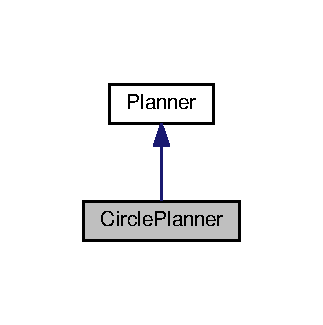
\includegraphics[width=155pt]{classCirclePlanner__inherit__graph}
\end{center}
\end{figure}


Collaboration diagram for Circle\+Planner\+:\nopagebreak
\begin{figure}[H]
\begin{center}
\leavevmode
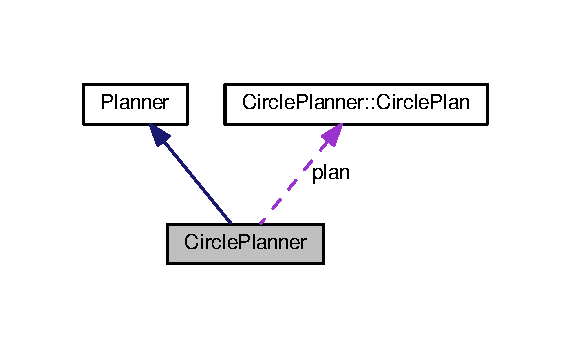
\includegraphics[width=274pt]{classCirclePlanner__coll__graph}
\end{center}
\end{figure}
\subsection*{Classes}
\begin{DoxyCompactItemize}
\item 
struct \hyperlink{structCirclePlanner_1_1CirclePlan}{Circle\+Plan}
\end{DoxyCompactItemize}
\subsection*{Public Member Functions}
\begin{DoxyCompactItemize}
\item 
{\bfseries Circle\+Planner} (ros\+::\+Node\+Handle \&\hyperlink{classPlanner_a9714d036f444a07ce90be8d135b9a40c}{nh})\hypertarget{classCirclePlanner_a33a27f97f5a1300d43c80b519fdfb3ef}{}\label{classCirclePlanner_a33a27f97f5a1300d43c80b519fdfb3ef}

\item 
void {\bfseries set\+\_\+parameter} (double r=3.\+0, double omega=0.\+5)\hypertarget{classCirclePlanner_a21fef783d5f2252fd1b53d93e869fc65}{}\label{classCirclePlanner_a21fef783d5f2252fd1b53d93e869fc65}

\item 
void {\bfseries load} ()\hypertarget{classCirclePlanner_a1c14f6ed36cbd32d39d60ed312a65de8}{}\label{classCirclePlanner_a1c14f6ed36cbd32d39d60ed312a65de8}

\end{DoxyCompactItemize}
\subsection*{Private Member Functions}
\begin{DoxyCompactItemize}
\item 
tf\+::\+Vector3 {\bfseries get\+\_\+position} (ros\+::\+Duration time)\hypertarget{classCirclePlanner_a1d6cdbec03a259af77937f0274dde5d9}{}\label{classCirclePlanner_a1d6cdbec03a259af77937f0274dde5d9}

\item 
tf\+::\+Quaternion {\bfseries get\+\_\+orientation} (ros\+::\+Duration time)\hypertarget{classCirclePlanner_a4e774b6cbc87a3dfa718df5594a0adbf}{}\label{classCirclePlanner_a4e774b6cbc87a3dfa718df5594a0adbf}

\item 
tf\+::\+Vector3 {\bfseries get\+\_\+velocity} (ros\+::\+Duration time)\hypertarget{classCirclePlanner_a5184277b2e174515140514fdec37ba29}{}\label{classCirclePlanner_a5184277b2e174515140514fdec37ba29}

\item 
double {\bfseries get\+\_\+angular\+\_\+velocity} (ros\+::\+Duration time)\hypertarget{classCirclePlanner_afa7c8502da92a63c78711ca92e73fe2b}{}\label{classCirclePlanner_afa7c8502da92a63c78711ca92e73fe2b}

\item 
void {\bfseries check\+\_\+period} (ros\+::\+Duration time)\hypertarget{classCirclePlanner_ab981788d76132e3f03ebedeb128d703a}{}\label{classCirclePlanner_ab981788d76132e3f03ebedeb128d703a}

\end{DoxyCompactItemize}
\subsection*{Private Attributes}
\begin{DoxyCompactItemize}
\item 
\hyperlink{structCirclePlanner_1_1CirclePlan}{Circle\+Plan} {\bfseries plan}\hypertarget{classCirclePlanner_a69f9e183351ef2c5325eef292350fb52}{}\label{classCirclePlanner_a69f9e183351ef2c5325eef292350fb52}

\end{DoxyCompactItemize}
\subsection*{Additional Inherited Members}


The documentation for this class was generated from the following files\+:\begin{DoxyCompactItemize}
\item 
simulation\+\_\+env/include/simulation\+\_\+env/planner.\+h\item 
simulation\+\_\+env/src/planner.\+cpp\end{DoxyCompactItemize}

\hypertarget{classController}{}\section{Controller Class Reference}
\label{classController}\index{Controller@{Controller}}


Provides a easy to use implementation of a generic mobile robot controller.  




{\ttfamily \#include $<$controller.\+h$>$}



Inheritance diagram for Controller\+:
\nopagebreak
\begin{figure}[H]
\begin{center}
\leavevmode
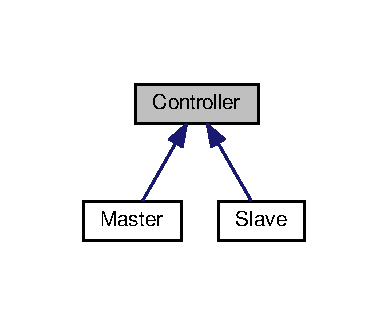
\includegraphics[width=186pt]{classController__inherit__graph}
\end{center}
\end{figure}


Collaboration diagram for Controller\+:\nopagebreak
\begin{figure}[H]
\begin{center}
\leavevmode
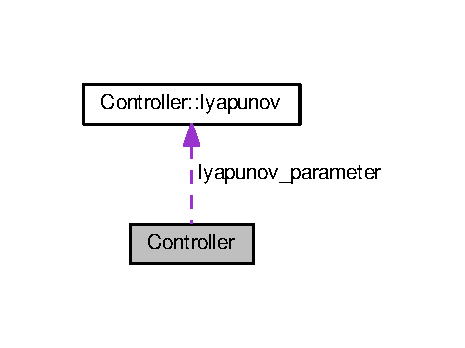
\includegraphics[width=350pt]{classController__coll__graph}
\end{center}
\end{figure}
\subsection*{Classes}
\begin{DoxyCompactItemize}
\item 
struct \hyperlink{structController_1_1ControlState}{Control\+State}
\begin{DoxyCompactList}\small\item\em Holds the System state combined by the pose of the system, the cartesian velocity and the angular velocity. \end{DoxyCompactList}\item 
struct \hyperlink{structController_1_1ControlVector}{Control\+Vector}
\begin{DoxyCompactList}\small\item\em A struct that holds linear and angular velocity of the Robot since this are the control variable for kinematic tracking control. \end{DoxyCompactList}\item 
struct \hyperlink{structController_1_1LyapunovParameter}{Lyapunov\+Parameter}
\begin{DoxyCompactList}\small\item\em Specifies the parameters needed for the lyapunov based control law. \end{DoxyCompactList}\end{DoxyCompactItemize}
\subsection*{Public Types}
\begin{DoxyCompactItemize}
\item 
enum \hyperlink{classController_aa6d956c4c220461a4152415ffa78690a}{Controller\+Type} \{ \hyperlink{classController_aa6d956c4c220461a4152415ffa78690aad2e9073ef821965020410686a3c89483}{pseudo\+\_\+inverse} =1, 
\hyperlink{classController_aa6d956c4c220461a4152415ffa78690aaed0e850e561d54619d85f32c37f5bfab}{lypanov} =2, 
\hyperlink{classController_aa6d956c4c220461a4152415ffa78690aa7ab0ee34114a951d4491d6eb73500cdc}{angle\+\_\+distance} =3
 \}\begin{DoxyCompactList}\small\item\em Specifies the different implemented control laws. \end{DoxyCompactList}
\item 
typedef tf\+::\+Vector3 \hyperlink{classController_a7ab3d947ee649f6bac652de6a00e8148}{Velocity\+Cartesian}\hypertarget{classController_a7ab3d947ee649f6bac652de6a00e8148}{}\label{classController_a7ab3d947ee649f6bac652de6a00e8148}

\begin{DoxyCompactList}\small\item\em Defines Velocity\+Cartesian wich is used to stores cartesian defined velocities. \end{DoxyCompactList}\item 
typedef tf\+::\+Vector3 \hyperlink{classController_a1b8b4035525237f0112b81d44a23da2c}{Position\+Cartesian}\hypertarget{classController_a1b8b4035525237f0112b81d44a23da2c}{}\label{classController_a1b8b4035525237f0112b81d44a23da2c}

\begin{DoxyCompactList}\small\item\em Defines Position\+Cartesian wich is used to store a cartesian defined position. \end{DoxyCompactList}\item 
typedef tf\+::\+Transform \hyperlink{classController_a75a1e2f93842f65d1263f7d3c2fd8898}{Control\+Difference}\hypertarget{classController_a75a1e2f93842f65d1263f7d3c2fd8898}{}\label{classController_a75a1e2f93842f65d1263f7d3c2fd8898}

\begin{DoxyCompactList}\small\item\em Defines Control\+Difference wich is a transformation from the current state in the target state. \end{DoxyCompactList}\item 
typedef \hyperlink{structController_1_1ControlVector}{Control\+Vector} \hyperlink{classController_a6849bee332c04d67ac6f3052cccd2669}{Velocity\+Eulerian}\hypertarget{classController_a6849bee332c04d67ac6f3052cccd2669}{}\label{classController_a6849bee332c04d67ac6f3052cccd2669}

\begin{DoxyCompactList}\small\item\em Defines Velocity\+Eulerian wich is used to store Velocities wich are defined locally in the moved base system. \end{DoxyCompactList}\end{DoxyCompactItemize}
\subsection*{Public Member Functions}
\begin{DoxyCompactItemize}
\item 
\hyperlink{classController_a7341f9092e1977cdd2a1492c4422c019}{Controller} (ros\+::\+Node\+Handle \&\hyperlink{classController_a24e3d3c2536f6ed29018bad1fd53dae2}{nh})
\begin{DoxyCompactList}\small\item\em Construct a new \hyperlink{classController}{Controller} object. \end{DoxyCompactList}\item 
\hyperlink{classController_a0ab87934c4f7a266cfdb86e0f36bc1b5}{$\sim$\+Controller} ()\hypertarget{classController_a0ab87934c4f7a266cfdb86e0f36bc1b5}{}\label{classController_a0ab87934c4f7a266cfdb86e0f36bc1b5}

\begin{DoxyCompactList}\small\item\em Destroy the \hyperlink{classController}{Controller} object. \end{DoxyCompactList}\item 
void \hyperlink{classController_a177d0d6cd7cdb7784ae9c506debfa2c6}{set\+Name} (std\+::string \hyperlink{classController_af81f22d8b64d915769acfb8e8d89e0c8}{name})
\begin{DoxyCompactList}\small\item\em Set the name of object. \end{DoxyCompactList}\item 
void \hyperlink{classController_a156a66bd7cd6340106accbb982b6238b}{set\+Reference} (double x, double y, double z, double angle)
\begin{DoxyCompactList}\small\item\em Set the reference of the mobile robot to be controlled from a global frame. \end{DoxyCompactList}\item 
void \hyperlink{classController_ae86ed49c452a9e94568312ef743aa082}{set\+Reference} (std\+::vector$<$ double $>$ coord, double angle)
\begin{DoxyCompactList}\small\item\em Set the reference of the mobile robot to be controlled from a global frame. \end{DoxyCompactList}\item 
void \hyperlink{classController_adf25339eadd9b31bc1d6b3e47395942e}{set\+World\+Frame} (std\+::string frame)
\begin{DoxyCompactList}\small\item\em Set the world frame name all references are given in. \end{DoxyCompactList}\item 
void \hyperlink{classController_a25202c469ad65696761242dce4e28d76}{set\+Type} (\hyperlink{classController_aa6d956c4c220461a4152415ffa78690a}{Controller\+::\+Controller\+Type} \hyperlink{classController_a17792cff397dc69baca568c7d03f2fc8}{type})
\begin{DoxyCompactList}\small\item\em Sets the type of the used control law. \end{DoxyCompactList}\item 
void \hyperlink{classController_abda96416fab439c188ef494a2b2a0c8e}{set\+Lyapunov} (\hyperlink{structController_1_1LyapunovParameter}{Controller\+::\+Lyapunov\+Parameter} param)
\begin{DoxyCompactList}\small\item\em Sets the parameter of the lyapunov control law. \end{DoxyCompactList}\item 
void \hyperlink{classController_a1f77caed7a7951ca2f4cf7928f88669d}{set\+Lyapunov} (std\+::vector$<$ float $>$ param)
\begin{DoxyCompactList}\small\item\em Sets the parameter of the lyapunov control law. \end{DoxyCompactList}\item 
virtual void \hyperlink{classController_a59e60885d5307979faf477435507069a}{load\+Parameter} ()\hypertarget{classController_a59e60885d5307979faf477435507069a}{}\label{classController_a59e60885d5307979faf477435507069a}

\begin{DoxyCompactList}\small\item\em Loading parameter for a specified \hyperlink{classController}{Controller}. Empty for \hyperlink{classController}{Controller} base class and implemented in inheriting classes. \end{DoxyCompactList}\item 
void \hyperlink{classController_a55c77d2e41634c9b21543647f74eec4c}{load} ()\hypertarget{classController_a55c77d2e41634c9b21543647f74eec4c}{}\label{classController_a55c77d2e41634c9b21543647f74eec4c}

\begin{DoxyCompactList}\small\item\em Loading of R\+OS parameterset for this controller. \end{DoxyCompactList}\item 
void \hyperlink{classController_aa0ea10adc7a81124663fb01693acef17}{link\+Current\+Odom} (std\+::string topic\+\_\+name)
\begin{DoxyCompactList}\small\item\em Links the current odometry topic to the controller. At this topic the current odomotry of the robot must be published. \end{DoxyCompactList}\item 
void \hyperlink{classController_a633d84f97952551654ee70acc31810c6}{link\+Target\+Odom} (std\+::string topic\+\_\+name)
\begin{DoxyCompactList}\small\item\em Links the target/desired odometry topic to the controller. At this topic the desired odometry is published. \end{DoxyCompactList}\item 
void \hyperlink{classController_a7bde6b39b2b2cccb1dd866841f672f99}{link\+Output\+Velocity} (std\+::string topic\+\_\+name)
\begin{DoxyCompactList}\small\item\em Links the output velocity of the controller to a given topic. \end{DoxyCompactList}\item 
void \hyperlink{classController_a6412541600d7444f00f8e48cea0ed024}{link\+Output\+Control\+Data} (std\+::string topic\+\_\+name)
\begin{DoxyCompactList}\small\item\em Links the meta data of the controller to a given topic. \end{DoxyCompactList}\item 
virtual void \hyperlink{classController_a9bf99e0d40660b832c2e70691e9f0a1c}{current\+Odom\+Callback} (nav\+\_\+msgs\+::\+Odometry msg)
\begin{DoxyCompactList}\small\item\em Callback for incoming odometry data for the current robot odometry. \end{DoxyCompactList}\item 
virtual void \hyperlink{classController_a77f138b6a3699c21cf904041e7e19820}{target\+Odom\+Callback} (nav\+\_\+msgs\+::\+Odometry msg)
\begin{DoxyCompactList}\small\item\em Callback for incoming state data for the target odometry of the robot. This is overloaded by child classes. \end{DoxyCompactList}\item 
struct \hyperlink{structController_1_1ControlVector}{Control\+Vector} \hyperlink{classController_a5342dd66c1228e651e569d9b1c31d82e}{calc\+Lyapunov} (\hyperlink{structController_1_1LyapunovParameter}{Lyapunov\+Parameter} parameter, \hyperlink{classController_a6849bee332c04d67ac6f3052cccd2669}{Velocity\+Eulerian} desired, tf\+::\+Transform relative)
\item 
void \hyperlink{classController_abe0a6e0155a0b159efe425e635d3ae76}{execute} (const ros\+::\+Timer\+Event \&ev)\hypertarget{classController_abe0a6e0155a0b159efe425e635d3ae76}{}\label{classController_abe0a6e0155a0b159efe425e635d3ae76}

\begin{DoxyCompactList}\small\item\em Scope of the controller that is called in control frequence. \end{DoxyCompactList}\item 
void \hyperlink{classController_ab5515748f1b0c82f015e039c817ee5f7}{reset} ()\hypertarget{classController_ab5515748f1b0c82f015e039c817ee5f7}{}\label{classController_ab5515748f1b0c82f015e039c817ee5f7}

\begin{DoxyCompactList}\small\item\em Resetting controller to initial state. \end{DoxyCompactList}\item 
bool \hyperlink{classController_a140aa1ee895337d776f88682640c0746}{srv\+Reset} (std\+\_\+srvs\+::\+Empty\+Request \&req, std\+\_\+srvs\+::\+Empty\+Response \&res)
\begin{DoxyCompactList}\small\item\em Service procedure for resetting the \hyperlink{classController}{Controller}. \end{DoxyCompactList}\item 
void \hyperlink{classController_a753fe3680abc7c9ba3040f6fcb638ac2}{control\+State2control\+State\+Msg} (\hyperlink{structController_1_1ControlState}{Control\+State} \&state, multi\+\_\+robot\+\_\+msgs\+::\+Control\+State \&msg)
\begin{DoxyCompactList}\small\item\em Converts \hyperlink{structController_1_1ControlState}{Control\+State} struct to a C\+Ontrol state message. \end{DoxyCompactList}\item 
void \hyperlink{classController_a866cee7328e1318e118c884a850a0e34}{control\+Difference2control\+Difference\+Msg} (\hyperlink{classController_a75a1e2f93842f65d1263f7d3c2fd8898}{Control\+Difference} \&difference, multi\+\_\+robot\+\_\+msgs\+::\+Control\+Difference \&msg)
\begin{DoxyCompactList}\small\item\em Converts Control\+Difference struct to a C\+Ontrol state message. \end{DoxyCompactList}\item 
void \hyperlink{classController_a06c1aab700c5918b76e33c35f3da8ea8}{control\+Vector2control\+Vector\+Msg} (\hyperlink{structController_1_1ControlVector}{Control\+Vector} \&control, multi\+\_\+robot\+\_\+msgs\+::\+Control\+Vector \&msg)
\begin{DoxyCompactList}\small\item\em Converts \hyperlink{structController_1_1ControlVector}{Control\+Vector} struct to a C\+Ontrol state message. \end{DoxyCompactList}\end{DoxyCompactItemize}
\subsection*{Protected Attributes}
\begin{DoxyCompactItemize}
\item 
ros\+::\+Node\+Handle \hyperlink{classController_a24e3d3c2536f6ed29018bad1fd53dae2}{nh}\hypertarget{classController_a24e3d3c2536f6ed29018bad1fd53dae2}{}\label{classController_a24e3d3c2536f6ed29018bad1fd53dae2}

\begin{DoxyCompactList}\small\item\em Node Handle. \end{DoxyCompactList}\item 
tf\+::\+Transform\+Listener $\ast$ \hyperlink{classController_afea373f808d583e4ad613f119439a8f5}{listener}\hypertarget{classController_afea373f808d583e4ad613f119439a8f5}{}\label{classController_afea373f808d583e4ad613f119439a8f5}

\begin{DoxyCompactList}\small\item\em Listener for any transformation. \end{DoxyCompactList}\item 
std\+::string \hyperlink{classController_ae01171e69d9b735e44964662275fc77c}{world\+\_\+frame}\hypertarget{classController_ae01171e69d9b735e44964662275fc77c}{}\label{classController_ae01171e69d9b735e44964662275fc77c}

\begin{DoxyCompactList}\small\item\em Name of the world frame. \end{DoxyCompactList}\item 
\hyperlink{structController_1_1ControlState}{Control\+State} \hyperlink{classController_aaca736f25e7da33272ded507e0c8057f}{current\+\_\+state\+\_\+}\hypertarget{classController_aaca736f25e7da33272ded507e0c8057f}{}\label{classController_aaca736f25e7da33272ded507e0c8057f}

\begin{DoxyCompactList}\small\item\em The current state of the robot. \end{DoxyCompactList}\item 
\hyperlink{structController_1_1ControlState}{Control\+State} \hyperlink{classController_a8412c8448970cf820f932cff02d69d33}{target\+\_\+state\+\_\+}\hypertarget{classController_a8412c8448970cf820f932cff02d69d33}{}\label{classController_a8412c8448970cf820f932cff02d69d33}

\begin{DoxyCompactList}\small\item\em The target state of the robot. \end{DoxyCompactList}\item 
\hyperlink{classController_a75a1e2f93842f65d1263f7d3c2fd8898}{Control\+Difference} \hyperlink{classController_afe3b54c59a80046661f0030a573539d7}{control\+\_\+dif\+\_\+}\hypertarget{classController_afe3b54c59a80046661f0030a573539d7}{}\label{classController_afe3b54c59a80046661f0030a573539d7}

\begin{DoxyCompactList}\small\item\em Transformation from current configuration to target configuration. \end{DoxyCompactList}\item 
\hyperlink{structController_1_1ControlVector}{Control\+Vector} \hyperlink{classController_aaafcd892e9e6080e839a1348a7ef40db}{control\+\_\+}\hypertarget{classController_aaafcd892e9e6080e839a1348a7ef40db}{}\label{classController_aaafcd892e9e6080e839a1348a7ef40db}

\begin{DoxyCompactList}\small\item\em The calculated control vector. \end{DoxyCompactList}\item 
tf\+::\+Transform \hyperlink{classController_aa713beca2ef8152d273bbc6fc38f7fc8}{world2reference\+\_\+}\hypertarget{classController_aa713beca2ef8152d273bbc6fc38f7fc8}{}\label{classController_aa713beca2ef8152d273bbc6fc38f7fc8}

\begin{DoxyCompactList}\small\item\em Transformation from a world to the controllers refrence frame. \end{DoxyCompactList}\end{DoxyCompactItemize}
\subsection*{Private Member Functions}
\begin{DoxyCompactItemize}
\item 
void \hyperlink{classController_ae6859e3a43be2fa31cb82ace3954e746}{publish} ()\hypertarget{classController_ae6859e3a43be2fa31cb82ace3954e746}{}\label{classController_ae6859e3a43be2fa31cb82ace3954e746}

\begin{DoxyCompactList}\small\item\em Publish all outgoing data. \end{DoxyCompactList}\item 
void \hyperlink{classController_a8509c67c73d26e981ef0972f44dc73ca}{publish\+\_\+refrence} ()\hypertarget{classController_a8509c67c73d26e981ef0972f44dc73ca}{}\label{classController_a8509c67c73d26e981ef0972f44dc73ca}

\begin{DoxyCompactList}\small\item\em Adding the world frame. Broadcastes a world frame respectiveliy the robot reference frame expressed in world coordinates. \end{DoxyCompactList}\end{DoxyCompactItemize}
\subsection*{Private Attributes}
\begin{DoxyCompactItemize}
\item 
ros\+::\+Publisher \hyperlink{classController_a2ff92c110ca7f28bdd702229a1295505}{pub\+\_\+cmd\+\_\+vel}\hypertarget{classController_a2ff92c110ca7f28bdd702229a1295505}{}\label{classController_a2ff92c110ca7f28bdd702229a1295505}

\begin{DoxyCompactList}\small\item\em publisher object for velocity outoput topic \end{DoxyCompactList}\item 
ros\+::\+Publisher \hyperlink{classController_a6abeaf23d1c17d6af6eecf7d1479fe31}{pub\+\_\+state\+\_\+out}\hypertarget{classController_a6abeaf23d1c17d6af6eecf7d1479fe31}{}\label{classController_a6abeaf23d1c17d6af6eecf7d1479fe31}

\begin{DoxyCompactList}\small\item\em publisher object for state output topic \end{DoxyCompactList}\item 
ros\+::\+Publisher \hyperlink{classController_afde3eefcf7ac040b2a38a8d1e95a6077}{pub\+\_\+control\+\_\+data}\hypertarget{classController_afde3eefcf7ac040b2a38a8d1e95a6077}{}\label{classController_afde3eefcf7ac040b2a38a8d1e95a6077}

\begin{DoxyCompactList}\small\item\em publisher object for control difference topic \end{DoxyCompactList}\item 
ros\+::\+Subscriber \hyperlink{classController_a855093341ac8afa84efd841654fedaf5}{sub\+\_\+odom\+\_\+current}\hypertarget{classController_a855093341ac8afa84efd841654fedaf5}{}\label{classController_a855093341ac8afa84efd841654fedaf5}

\begin{DoxyCompactList}\small\item\em Subscriber object for odometry. \end{DoxyCompactList}\item 
ros\+::\+Subscriber \hyperlink{classController_a7c21cd887b80a3ebceae1e5e320c6ad8}{sub\+\_\+odom\+\_\+target}\hypertarget{classController_a7c21cd887b80a3ebceae1e5e320c6ad8}{}\label{classController_a7c21cd887b80a3ebceae1e5e320c6ad8}

\begin{DoxyCompactList}\small\item\em Subscriber object for target odometry topic. \end{DoxyCompactList}\item 
ros\+::\+Timer \hyperlink{classController_a96e34ca6ebe5b7c8035982ff98270f4b}{time\+\_\+scope\+\_\+}\hypertarget{classController_a96e34ca6ebe5b7c8035982ff98270f4b}{}\label{classController_a96e34ca6ebe5b7c8035982ff98270f4b}

\begin{DoxyCompactList}\small\item\em Timer for control scope. \end{DoxyCompactList}\item 
ros\+::\+Service\+Server \hyperlink{classController_ae981013bac649b6310e924b6a126bc40}{reset\+\_\+service}\hypertarget{classController_ae981013bac649b6310e924b6a126bc40}{}\label{classController_ae981013bac649b6310e924b6a126bc40}

\begin{DoxyCompactList}\small\item\em Service for resetting the controller. \end{DoxyCompactList}\item 
std\+::string \hyperlink{classController_af81f22d8b64d915769acfb8e8d89e0c8}{name}\hypertarget{classController_af81f22d8b64d915769acfb8e8d89e0c8}{}\label{classController_af81f22d8b64d915769acfb8e8d89e0c8}

\begin{DoxyCompactList}\small\item\em Name of the node respective \hyperlink{classController}{Controller}. \end{DoxyCompactList}\item 
\hyperlink{structController_1_1LyapunovParameter}{Lyapunov\+Parameter} \hyperlink{classController_a8069db2319ff64d65607b1aa897d3069}{lyapunov\+\_\+parameter}\hypertarget{classController_a8069db2319ff64d65607b1aa897d3069}{}\label{classController_a8069db2319ff64d65607b1aa897d3069}

\begin{DoxyCompactList}\small\item\em Parameter set for lyapunov determinations. \end{DoxyCompactList}\item 
\hyperlink{classController_aa6d956c4c220461a4152415ffa78690a}{Controller\+Type} \hyperlink{classController_a17792cff397dc69baca568c7d03f2fc8}{type}\hypertarget{classController_a17792cff397dc69baca568c7d03f2fc8}{}\label{classController_a17792cff397dc69baca568c7d03f2fc8}

\begin{DoxyCompactList}\small\item\em Type of control algorythm that is used. \end{DoxyCompactList}\item 
bool \hyperlink{classController_a4e0e569456498e5670a48244c22cafc9}{loaded\+\_\+parameter}\hypertarget{classController_a4e0e569456498e5670a48244c22cafc9}{}\label{classController_a4e0e569456498e5670a48244c22cafc9}

\begin{DoxyCompactList}\small\item\em Flag if parameter were loaded from the parameter server. \end{DoxyCompactList}\end{DoxyCompactItemize}


\subsection{Detailed Description}
Provides a easy to use implementation of a generic mobile robot controller. 

\subsection{Member Enumeration Documentation}
\index{Controller@{Controller}!Controller\+Type@{Controller\+Type}}
\index{Controller\+Type@{Controller\+Type}!Controller@{Controller}}
\subsubsection[{\texorpdfstring{Controller\+Type}{ControllerType}}]{\setlength{\rightskip}{0pt plus 5cm}enum {\bf Controller\+::\+Controller\+Type}}\hypertarget{classController_aa6d956c4c220461a4152415ffa78690a}{}\label{classController_aa6d956c4c220461a4152415ffa78690a}


Specifies the different implemented control laws. 

\begin{Desc}
\item[Enumerator]\par
\begin{description}
\index{pseudo\+\_\+inverse@{pseudo\+\_\+inverse}!Controller@{Controller}}\index{Controller@{Controller}!pseudo\+\_\+inverse@{pseudo\+\_\+inverse}}\item[{\em 
pseudo\+\_\+inverse\hypertarget{classController_aa6d956c4c220461a4152415ffa78690aad2e9073ef821965020410686a3c89483}{}\label{classController_aa6d956c4c220461a4152415ffa78690aad2e9073ef821965020410686a3c89483}
}]Control law is based on pseudo inveres the input for generate a output (least squares optimisation) \index{lypanov@{lypanov}!Controller@{Controller}}\index{Controller@{Controller}!lypanov@{lypanov}}\item[{\em 
lypanov\hypertarget{classController_aa6d956c4c220461a4152415ffa78690aaed0e850e561d54619d85f32c37f5bfab}{}\label{classController_aa6d956c4c220461a4152415ffa78690aaed0e850e561d54619d85f32c37f5bfab}
}]Control law is based on the lyapunov approache. Output is determined from a lyapunov stable function \index{angle\+\_\+distance@{angle\+\_\+distance}!Controller@{Controller}}\index{Controller@{Controller}!angle\+\_\+distance@{angle\+\_\+distance}}\item[{\em 
angle\+\_\+distance\hypertarget{classController_aa6d956c4c220461a4152415ffa78690aa7ab0ee34114a951d4491d6eb73500cdc}{}\label{classController_aa6d956c4c220461a4152415ffa78690aa7ab0ee34114a951d4491d6eb73500cdc}
}]Control law based on linear approach in angle and distance respectively \end{description}
\end{Desc}


\subsection{Constructor \& Destructor Documentation}
\index{Controller@{Controller}!Controller@{Controller}}
\index{Controller@{Controller}!Controller@{Controller}}
\subsubsection[{\texorpdfstring{Controller(ros\+::\+Node\+Handle \&nh)}{Controller(ros::NodeHandle &nh)}}]{\setlength{\rightskip}{0pt plus 5cm}Controller\+::\+Controller (
\begin{DoxyParamCaption}
\item[{ros\+::\+Node\+Handle \&}]{nh}
\end{DoxyParamCaption}
)}\hypertarget{classController_a7341f9092e1977cdd2a1492c4422c019}{}\label{classController_a7341f9092e1977cdd2a1492c4422c019}


Construct a new \hyperlink{classController}{Controller} object. 


\begin{DoxyParams}{Parameters}
{\em nh} & Ros nodehandle for managing namespaces and ros functionality within the controller object \\
\hline
\end{DoxyParams}


\subsection{Member Function Documentation}
\index{Controller@{Controller}!calc\+Lyapunov@{calc\+Lyapunov}}
\index{calc\+Lyapunov@{calc\+Lyapunov}!Controller@{Controller}}
\subsubsection[{\texorpdfstring{calc\+Lyapunov(\+Lyapunov\+Parameter parameter, Velocity\+Eulerian desired, tf\+::\+Transform relative)}{calcLyapunov(LyapunovParameter parameter, VelocityEulerian desired, tf::Transform relative)}}]{\setlength{\rightskip}{0pt plus 5cm}struct {\bf Controller\+::\+Control\+Vector} Controller\+::calc\+Lyapunov (
\begin{DoxyParamCaption}
\item[{{\bf Lyapunov\+Parameter}}]{parameter, }
\item[{{\bf Velocity\+Eulerian}}]{desired, }
\item[{tf\+::\+Transform}]{relative}
\end{DoxyParamCaption}
)}\hypertarget{classController_a5342dd66c1228e651e569d9b1c31d82e}{}\label{classController_a5342dd66c1228e651e569d9b1c31d82e}

\begin{DoxyParams}{Parameters}
{\em parameter} & Set of lyapunov parameter for calculating the control vector \\
\hline
{\em desired} & Desired velocities in eulerian description (moved base). Contains angular and linear velocity \\
\hline
{\em relative} & Transformation from current to target state \\
\hline
\end{DoxyParams}
\begin{DoxyReturn}{Returns}
\hyperlink{structController_1_1ControlVector}{Control\+Vector} 
\end{DoxyReturn}
\index{Controller@{Controller}!control\+Difference2control\+Difference\+Msg@{control\+Difference2control\+Difference\+Msg}}
\index{control\+Difference2control\+Difference\+Msg@{control\+Difference2control\+Difference\+Msg}!Controller@{Controller}}
\subsubsection[{\texorpdfstring{control\+Difference2control\+Difference\+Msg(\+Control\+Difference \&difference, multi\+\_\+robot\+\_\+msgs\+::\+Control\+Difference \&msg)}{controlDifference2controlDifferenceMsg(ControlDifference &difference, multi_robot_msgs::ControlDifference &msg)}}]{\setlength{\rightskip}{0pt plus 5cm}void Controller\+::control\+Difference2control\+Difference\+Msg (
\begin{DoxyParamCaption}
\item[{{\bf Control\+Difference} \&}]{difference, }
\item[{multi\+\_\+robot\+\_\+msgs\+::\+Control\+Difference \&}]{msg}
\end{DoxyParamCaption}
)}\hypertarget{classController_a866cee7328e1318e118c884a850a0e34}{}\label{classController_a866cee7328e1318e118c884a850a0e34}


Converts Control\+Difference struct to a C\+Ontrol state message. 


\begin{DoxyParams}{Parameters}
{\em difference} & Control\+Difference to be converted \\
\hline
{\em msg} & Referenze to the msg the conversion is stored in \\
\hline
\end{DoxyParams}
\index{Controller@{Controller}!control\+State2control\+State\+Msg@{control\+State2control\+State\+Msg}}
\index{control\+State2control\+State\+Msg@{control\+State2control\+State\+Msg}!Controller@{Controller}}
\subsubsection[{\texorpdfstring{control\+State2control\+State\+Msg(\+Control\+State \&state, multi\+\_\+robot\+\_\+msgs\+::\+Control\+State \&msg)}{controlState2controlStateMsg(ControlState &state, multi_robot_msgs::ControlState &msg)}}]{\setlength{\rightskip}{0pt plus 5cm}void Controller\+::control\+State2control\+State\+Msg (
\begin{DoxyParamCaption}
\item[{{\bf Controller\+::\+Control\+State} \&}]{state, }
\item[{multi\+\_\+robot\+\_\+msgs\+::\+Control\+State \&}]{msg}
\end{DoxyParamCaption}
)}\hypertarget{classController_a753fe3680abc7c9ba3040f6fcb638ac2}{}\label{classController_a753fe3680abc7c9ba3040f6fcb638ac2}


Converts \hyperlink{structController_1_1ControlState}{Control\+State} struct to a C\+Ontrol state message. 


\begin{DoxyParams}{Parameters}
{\em state} & Control state to be converted \\
\hline
{\em msg} & Referenze to the msg the conversion is stored in \\
\hline
\end{DoxyParams}
\index{Controller@{Controller}!control\+Vector2control\+Vector\+Msg@{control\+Vector2control\+Vector\+Msg}}
\index{control\+Vector2control\+Vector\+Msg@{control\+Vector2control\+Vector\+Msg}!Controller@{Controller}}
\subsubsection[{\texorpdfstring{control\+Vector2control\+Vector\+Msg(\+Control\+Vector \&control, multi\+\_\+robot\+\_\+msgs\+::\+Control\+Vector \&msg)}{controlVector2controlVectorMsg(ControlVector &control, multi_robot_msgs::ControlVector &msg)}}]{\setlength{\rightskip}{0pt plus 5cm}void Controller\+::control\+Vector2control\+Vector\+Msg (
\begin{DoxyParamCaption}
\item[{{\bf Control\+Vector} \&}]{control, }
\item[{multi\+\_\+robot\+\_\+msgs\+::\+Control\+Vector \&}]{msg}
\end{DoxyParamCaption}
)}\hypertarget{classController_a06c1aab700c5918b76e33c35f3da8ea8}{}\label{classController_a06c1aab700c5918b76e33c35f3da8ea8}


Converts \hyperlink{structController_1_1ControlVector}{Control\+Vector} struct to a C\+Ontrol state message. 


\begin{DoxyParams}{Parameters}
{\em control} & \hyperlink{structController_1_1ControlVector}{Control\+Vector} to be converted \\
\hline
{\em msg} & Referenze to the msg the conversion is stored in \\
\hline
\end{DoxyParams}
\index{Controller@{Controller}!current\+Odom\+Callback@{current\+Odom\+Callback}}
\index{current\+Odom\+Callback@{current\+Odom\+Callback}!Controller@{Controller}}
\subsubsection[{\texorpdfstring{current\+Odom\+Callback(nav\+\_\+msgs\+::\+Odometry msg)}{currentOdomCallback(nav_msgs::Odometry msg)}}]{\setlength{\rightskip}{0pt plus 5cm}void Controller\+::current\+Odom\+Callback (
\begin{DoxyParamCaption}
\item[{nav\+\_\+msgs\+::\+Odometry}]{msg}
\end{DoxyParamCaption}
)\hspace{0.3cm}{\ttfamily [virtual]}}\hypertarget{classController_a9bf99e0d40660b832c2e70691e9f0a1c}{}\label{classController_a9bf99e0d40660b832c2e70691e9f0a1c}


Callback for incoming odometry data for the current robot odometry. 


\begin{DoxyParams}{Parameters}
{\em msg} & Incoming message \\
\hline
\end{DoxyParams}
\index{Controller@{Controller}!link\+Current\+Odom@{link\+Current\+Odom}}
\index{link\+Current\+Odom@{link\+Current\+Odom}!Controller@{Controller}}
\subsubsection[{\texorpdfstring{link\+Current\+Odom(std\+::string topic\+\_\+name)}{linkCurrentOdom(std::string topic_name)}}]{\setlength{\rightskip}{0pt plus 5cm}void Controller\+::link\+Current\+Odom (
\begin{DoxyParamCaption}
\item[{std\+::string}]{topic\+\_\+name}
\end{DoxyParamCaption}
)}\hypertarget{classController_aa0ea10adc7a81124663fb01693acef17}{}\label{classController_aa0ea10adc7a81124663fb01693acef17}


Links the current odometry topic to the controller. At this topic the current odomotry of the robot must be published. 


\begin{DoxyParams}{Parameters}
{\em topic\+\_\+name} & Name of the topic \\
\hline
\end{DoxyParams}
\index{Controller@{Controller}!link\+Output\+Control\+Data@{link\+Output\+Control\+Data}}
\index{link\+Output\+Control\+Data@{link\+Output\+Control\+Data}!Controller@{Controller}}
\subsubsection[{\texorpdfstring{link\+Output\+Control\+Data(std\+::string topic\+\_\+name)}{linkOutputControlData(std::string topic_name)}}]{\setlength{\rightskip}{0pt plus 5cm}void Controller\+::link\+Output\+Control\+Data (
\begin{DoxyParamCaption}
\item[{std\+::string}]{topic\+\_\+name}
\end{DoxyParamCaption}
)}\hypertarget{classController_a6412541600d7444f00f8e48cea0ed024}{}\label{classController_a6412541600d7444f00f8e48cea0ed024}


Links the meta data of the controller to a given topic. 


\begin{DoxyParams}{Parameters}
{\em topic\+\_\+name} & Name of the topic \\
\hline
\end{DoxyParams}
\index{Controller@{Controller}!link\+Output\+Velocity@{link\+Output\+Velocity}}
\index{link\+Output\+Velocity@{link\+Output\+Velocity}!Controller@{Controller}}
\subsubsection[{\texorpdfstring{link\+Output\+Velocity(std\+::string topic\+\_\+name)}{linkOutputVelocity(std::string topic_name)}}]{\setlength{\rightskip}{0pt plus 5cm}void Controller\+::link\+Output\+Velocity (
\begin{DoxyParamCaption}
\item[{std\+::string}]{topic\+\_\+name}
\end{DoxyParamCaption}
)}\hypertarget{classController_a7bde6b39b2b2cccb1dd866841f672f99}{}\label{classController_a7bde6b39b2b2cccb1dd866841f672f99}


Links the output velocity of the controller to a given topic. 

O\+U\+T\+P\+U\+TS.


\begin{DoxyParams}{Parameters}
{\em topic\+\_\+name} & Name of the topic \\
\hline
\end{DoxyParams}
\index{Controller@{Controller}!link\+Target\+Odom@{link\+Target\+Odom}}
\index{link\+Target\+Odom@{link\+Target\+Odom}!Controller@{Controller}}
\subsubsection[{\texorpdfstring{link\+Target\+Odom(std\+::string topic\+\_\+name)}{linkTargetOdom(std::string topic_name)}}]{\setlength{\rightskip}{0pt plus 5cm}void Controller\+::link\+Target\+Odom (
\begin{DoxyParamCaption}
\item[{std\+::string}]{topic\+\_\+name}
\end{DoxyParamCaption}
)}\hypertarget{classController_a633d84f97952551654ee70acc31810c6}{}\label{classController_a633d84f97952551654ee70acc31810c6}


Links the target/desired odometry topic to the controller. At this topic the desired odometry is published. 


\begin{DoxyParams}{Parameters}
{\em topic\+\_\+name} & Name of the topic \\
\hline
\end{DoxyParams}
\index{Controller@{Controller}!set\+Lyapunov@{set\+Lyapunov}}
\index{set\+Lyapunov@{set\+Lyapunov}!Controller@{Controller}}
\subsubsection[{\texorpdfstring{set\+Lyapunov(\+Controller\+::\+Lyapunov\+Parameter param)}{setLyapunov(Controller::LyapunovParameter param)}}]{\setlength{\rightskip}{0pt plus 5cm}void Controller\+::set\+Lyapunov (
\begin{DoxyParamCaption}
\item[{{\bf Controller\+::\+Lyapunov\+Parameter}}]{param}
\end{DoxyParamCaption}
)}\hypertarget{classController_abda96416fab439c188ef494a2b2a0c8e}{}\label{classController_abda96416fab439c188ef494a2b2a0c8e}


Sets the parameter of the lyapunov control law. 


\begin{DoxyParams}{Parameters}
{\em param} & Parameterset as defined in lyapunov struct \\
\hline
\end{DoxyParams}
\index{Controller@{Controller}!set\+Lyapunov@{set\+Lyapunov}}
\index{set\+Lyapunov@{set\+Lyapunov}!Controller@{Controller}}
\subsubsection[{\texorpdfstring{set\+Lyapunov(std\+::vector$<$ float $>$ param)}{setLyapunov(std::vector< float > param)}}]{\setlength{\rightskip}{0pt plus 5cm}void Controller\+::set\+Lyapunov (
\begin{DoxyParamCaption}
\item[{std\+::vector$<$ float $>$}]{param}
\end{DoxyParamCaption}
)}\hypertarget{classController_a1f77caed7a7951ca2f4cf7928f88669d}{}\label{classController_a1f77caed7a7951ca2f4cf7928f88669d}


Sets the parameter of the lyapunov control law. 


\begin{DoxyParams}{Parameters}
{\em param} & vector of given parameters \mbox{[}kx,ky,ktheta,vd,omega\mbox{]} \\
\hline
\end{DoxyParams}
\index{Controller@{Controller}!set\+Name@{set\+Name}}
\index{set\+Name@{set\+Name}!Controller@{Controller}}
\subsubsection[{\texorpdfstring{set\+Name(std\+::string name)}{setName(std::string name)}}]{\setlength{\rightskip}{0pt plus 5cm}void Controller\+::set\+Name (
\begin{DoxyParamCaption}
\item[{std\+::string}]{name}
\end{DoxyParamCaption}
)}\hypertarget{classController_a177d0d6cd7cdb7784ae9c506debfa2c6}{}\label{classController_a177d0d6cd7cdb7784ae9c506debfa2c6}


Set the name of object. 


\begin{DoxyParams}{Parameters}
{\em name} & Name to be set \\
\hline
\end{DoxyParams}
\index{Controller@{Controller}!set\+Reference@{set\+Reference}}
\index{set\+Reference@{set\+Reference}!Controller@{Controller}}
\subsubsection[{\texorpdfstring{set\+Reference(double x, double y, double z, double angle)}{setReference(double x, double y, double z, double angle)}}]{\setlength{\rightskip}{0pt plus 5cm}void Controller\+::set\+Reference (
\begin{DoxyParamCaption}
\item[{double}]{x, }
\item[{double}]{y, }
\item[{double}]{z, }
\item[{double}]{angle}
\end{DoxyParamCaption}
)}\hypertarget{classController_a156a66bd7cd6340106accbb982b6238b}{}\label{classController_a156a66bd7cd6340106accbb982b6238b}


Set the reference of the mobile robot to be controlled from a global frame. 


\begin{DoxyParams}{Parameters}
{\em x} & X-\/position of robot \\
\hline
{\em y} & Y-\/position of robot \\
\hline
{\em z} & Z-\/position of robot \\
\hline
{\em angle} & Angular-\/position of robot \\
\hline
\end{DoxyParams}
\index{Controller@{Controller}!set\+Reference@{set\+Reference}}
\index{set\+Reference@{set\+Reference}!Controller@{Controller}}
\subsubsection[{\texorpdfstring{set\+Reference(std\+::vector$<$ double $>$ coord, double angle)}{setReference(std::vector< double > coord, double angle)}}]{\setlength{\rightskip}{0pt plus 5cm}void Controller\+::set\+Reference (
\begin{DoxyParamCaption}
\item[{std\+::vector$<$ double $>$}]{coord, }
\item[{double}]{angle}
\end{DoxyParamCaption}
)}\hypertarget{classController_ae86ed49c452a9e94568312ef743aa082}{}\label{classController_ae86ed49c452a9e94568312ef743aa082}


Set the reference of the mobile robot to be controlled from a global frame. 


\begin{DoxyParams}{Parameters}
{\em coord} & vector of the robot position \mbox{[}x,y,z\mbox{]} \\
\hline
{\em angle} & angel of the robot \\
\hline
\end{DoxyParams}
\index{Controller@{Controller}!set\+Type@{set\+Type}}
\index{set\+Type@{set\+Type}!Controller@{Controller}}
\subsubsection[{\texorpdfstring{set\+Type(\+Controller\+::\+Controller\+Type type)}{setType(Controller::ControllerType type)}}]{\setlength{\rightskip}{0pt plus 5cm}void Controller\+::set\+Type (
\begin{DoxyParamCaption}
\item[{{\bf Controller\+::\+Controller\+Type}}]{type}
\end{DoxyParamCaption}
)}\hypertarget{classController_a25202c469ad65696761242dce4e28d76}{}\label{classController_a25202c469ad65696761242dce4e28d76}


Sets the type of the used control law. 


\begin{DoxyParams}{Parameters}
{\em type} & Type of the controller as defined in controller\+Type \\
\hline
\end{DoxyParams}
\index{Controller@{Controller}!set\+World\+Frame@{set\+World\+Frame}}
\index{set\+World\+Frame@{set\+World\+Frame}!Controller@{Controller}}
\subsubsection[{\texorpdfstring{set\+World\+Frame(std\+::string frame)}{setWorldFrame(std::string frame)}}]{\setlength{\rightskip}{0pt plus 5cm}void Controller\+::set\+World\+Frame (
\begin{DoxyParamCaption}
\item[{std\+::string}]{frame}
\end{DoxyParamCaption}
)}\hypertarget{classController_adf25339eadd9b31bc1d6b3e47395942e}{}\label{classController_adf25339eadd9b31bc1d6b3e47395942e}


Set the world frame name all references are given in. 


\begin{DoxyParams}{Parameters}
{\em frame} & Name of the world frame \\
\hline
\end{DoxyParams}
\index{Controller@{Controller}!srv\+Reset@{srv\+Reset}}
\index{srv\+Reset@{srv\+Reset}!Controller@{Controller}}
\subsubsection[{\texorpdfstring{srv\+Reset(std\+\_\+srvs\+::\+Empty\+Request \&req, std\+\_\+srvs\+::\+Empty\+Response \&res)}{srvReset(std_srvs::EmptyRequest &req, std_srvs::EmptyResponse &res)}}]{\setlength{\rightskip}{0pt plus 5cm}bool Controller\+::srv\+Reset (
\begin{DoxyParamCaption}
\item[{std\+\_\+srvs\+::\+Empty\+Request \&}]{req, }
\item[{std\+\_\+srvs\+::\+Empty\+Response \&}]{res}
\end{DoxyParamCaption}
)}\hypertarget{classController_a140aa1ee895337d776f88682640c0746}{}\label{classController_a140aa1ee895337d776f88682640c0746}


Service procedure for resetting the \hyperlink{classController}{Controller}. 


\begin{DoxyParams}{Parameters}
{\em req} & Reqest for the service \\
\hline
{\em res} & Responce of the service \\
\hline
\end{DoxyParams}
\begin{DoxyReturn}{Returns}
true succeeded 

false not succeeded 
\end{DoxyReturn}
\index{Controller@{Controller}!target\+Odom\+Callback@{target\+Odom\+Callback}}
\index{target\+Odom\+Callback@{target\+Odom\+Callback}!Controller@{Controller}}
\subsubsection[{\texorpdfstring{target\+Odom\+Callback(nav\+\_\+msgs\+::\+Odometry msg)}{targetOdomCallback(nav_msgs::Odometry msg)}}]{\setlength{\rightskip}{0pt plus 5cm}void Controller\+::target\+Odom\+Callback (
\begin{DoxyParamCaption}
\item[{nav\+\_\+msgs\+::\+Odometry}]{msg}
\end{DoxyParamCaption}
)\hspace{0.3cm}{\ttfamily [virtual]}}\hypertarget{classController_a77f138b6a3699c21cf904041e7e19820}{}\label{classController_a77f138b6a3699c21cf904041e7e19820}


Callback for incoming state data for the target odometry of the robot. This is overloaded by child classes. 


\begin{DoxyParams}{Parameters}
{\em msg} & Incoming message \\
\hline
\end{DoxyParams}


Reimplemented in \hyperlink{classSlave_a2f80eae9dc8e4e20037c1a371f9b8189}{Slave}.



The documentation for this class was generated from the following files\+:\begin{DoxyCompactItemize}
\item 
controller/include/controller/controller.\+h\item 
controller/src/controller.\+cpp\end{DoxyCompactItemize}

\hypertarget{structController_1_1ControlState}{}\section{Controller\+:\+:Control\+State Struct Reference}
\label{structController_1_1ControlState}\index{Controller\+::\+Control\+State@{Controller\+::\+Control\+State}}


Holds the System state combined by the pose of the system, the cartesian velocity and the angular velocity.  




{\ttfamily \#include $<$controller.\+h$>$}

\subsection*{Public Member Functions}
\begin{DoxyCompactItemize}
\item 
\hyperlink{structController_1_1ControlState_a796d0aa1a726976960e68a9e4a81f535}{Control\+State} ()\hypertarget{structController_1_1ControlState_a796d0aa1a726976960e68a9e4a81f535}{}\label{structController_1_1ControlState_a796d0aa1a726976960e68a9e4a81f535}

\begin{DoxyCompactList}\small\item\em Construct a new Control State object with default memebers. \end{DoxyCompactList}\end{DoxyCompactItemize}
\subsection*{Public Attributes}
\begin{DoxyCompactItemize}
\item 
tf\+::\+Pose \hyperlink{structController_1_1ControlState_a7c5ccd93c34234a339675a8882007972}{pose}\hypertarget{structController_1_1ControlState_a7c5ccd93c34234a339675a8882007972}{}\label{structController_1_1ControlState_a7c5ccd93c34234a339675a8882007972}

\begin{DoxyCompactList}\small\item\em Complete pose of the robot in 3 dimensional space. \end{DoxyCompactList}\item 
\hyperlink{classController_a7ab3d947ee649f6bac652de6a00e8148}{Velocity\+Cartesian} \hyperlink{structController_1_1ControlState_a3555392a901189a545630300a7b71e67}{velocity}\hypertarget{structController_1_1ControlState_a3555392a901189a545630300a7b71e67}{}\label{structController_1_1ControlState_a3555392a901189a545630300a7b71e67}

\begin{DoxyCompactList}\small\item\em Velocity in cartesian space. \end{DoxyCompactList}\item 
double \hyperlink{structController_1_1ControlState_acb345c317b7389a4553f28252a6f66b5}{angular\+\_\+velocity}\hypertarget{structController_1_1ControlState_acb345c317b7389a4553f28252a6f66b5}{}\label{structController_1_1ControlState_acb345c317b7389a4553f28252a6f66b5}

\begin{DoxyCompactList}\small\item\em Angular velocity around z-\/axis. \end{DoxyCompactList}\end{DoxyCompactItemize}


\subsection{Detailed Description}
Holds the System state combined by the pose of the system, the cartesian velocity and the angular velocity. 

The documentation for this struct was generated from the following file\+:\begin{DoxyCompactItemize}
\item 
controller/include/controller/controller.\+h\end{DoxyCompactItemize}

\hypertarget{structController_1_1ControlVector}{}\section{Controller\+:\+:Control\+Vector Struct Reference}
\label{structController_1_1ControlVector}\index{Controller\+::\+Control\+Vector@{Controller\+::\+Control\+Vector}}


A struct that holds linear and angular velocity of the Robot since this are the control variable for kinematic tracking control.  




{\ttfamily \#include $<$controller.\+h$>$}

\subsection*{Public Member Functions}
\begin{DoxyCompactItemize}
\item 
\hyperlink{structController_1_1ControlVector_abf98db4ce95ac636bb5ac950b6b820b3}{Control\+Vector} ()\hypertarget{structController_1_1ControlVector_abf98db4ce95ac636bb5ac950b6b820b3}{}\label{structController_1_1ControlVector_abf98db4ce95ac636bb5ac950b6b820b3}

\begin{DoxyCompactList}\small\item\em Construct a new Control Vector object with default parameters. \end{DoxyCompactList}\end{DoxyCompactItemize}
\subsection*{Public Attributes}
\begin{DoxyCompactItemize}
\item 
double \hyperlink{structController_1_1ControlVector_af8d8ff93ddf343a13a35bba355d39976}{v}\hypertarget{structController_1_1ControlVector_af8d8ff93ddf343a13a35bba355d39976}{}\label{structController_1_1ControlVector_af8d8ff93ddf343a13a35bba355d39976}

\begin{DoxyCompactList}\small\item\em Linear velocity. \end{DoxyCompactList}\item 
double \hyperlink{structController_1_1ControlVector_ad5963169c4ea0c021cb923191aef7ed3}{omega}\hypertarget{structController_1_1ControlVector_ad5963169c4ea0c021cb923191aef7ed3}{}\label{structController_1_1ControlVector_ad5963169c4ea0c021cb923191aef7ed3}

\begin{DoxyCompactList}\small\item\em Angular velocity. \end{DoxyCompactList}\end{DoxyCompactItemize}


\subsection{Detailed Description}
A struct that holds linear and angular velocity of the Robot since this are the control variable for kinematic tracking control. 

The documentation for this struct was generated from the following file\+:\begin{DoxyCompactItemize}
\item 
controller/include/controller/controller.\+h\end{DoxyCompactItemize}

\hypertarget{structLissajousPlanner_1_1LissajousPlan}{}\section{Lissajous\+Planner\+:\+:Lissajous\+Plan Struct Reference}
\label{structLissajousPlanner_1_1LissajousPlan}\index{Lissajous\+Planner\+::\+Lissajous\+Plan@{Lissajous\+Planner\+::\+Lissajous\+Plan}}
\subsection*{Public Attributes}
\begin{DoxyCompactItemize}
\item 
float {\bfseries dphi}\hypertarget{structLissajousPlanner_1_1LissajousPlan_a60c6081d5506c1be5e0c4b48d5980b8d}{}\label{structLissajousPlanner_1_1LissajousPlan_a60c6081d5506c1be5e0c4b48d5980b8d}

\item 
float {\bfseries omegax}\hypertarget{structLissajousPlanner_1_1LissajousPlan_a54e05e3d4666b9843c13afe751d868e6}{}\label{structLissajousPlanner_1_1LissajousPlan_a54e05e3d4666b9843c13afe751d868e6}

\item 
int {\bfseries ratio}\hypertarget{structLissajousPlanner_1_1LissajousPlan_a1d7a8cb09570d913576d0b3592674e1f}{}\label{structLissajousPlanner_1_1LissajousPlan_a1d7a8cb09570d913576d0b3592674e1f}

\item 
float {\bfseries Ax}\hypertarget{structLissajousPlanner_1_1LissajousPlan_a85bedcfba3d78cb16bd67cc402b674ef}{}\label{structLissajousPlanner_1_1LissajousPlan_a85bedcfba3d78cb16bd67cc402b674ef}

\item 
float {\bfseries Ay}\hypertarget{structLissajousPlanner_1_1LissajousPlan_a72082318cebb55674e68a3383a81721f}{}\label{structLissajousPlanner_1_1LissajousPlan_a72082318cebb55674e68a3383a81721f}

\end{DoxyCompactItemize}


The documentation for this struct was generated from the following file\+:\begin{DoxyCompactItemize}
\item 
simulation\+\_\+env/include/simulation\+\_\+env/planner.\+h\end{DoxyCompactItemize}

\hypertarget{classLissajousPlanner}{}\section{Lissajous\+Planner Class Reference}
\label{classLissajousPlanner}\index{Lissajous\+Planner@{Lissajous\+Planner}}


Inheritance diagram for Lissajous\+Planner\+:\nopagebreak
\begin{figure}[H]
\begin{center}
\leavevmode
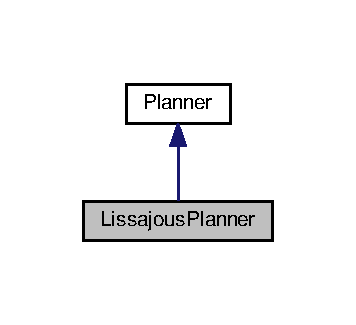
\includegraphics[width=171pt]{classLissajousPlanner__inherit__graph}
\end{center}
\end{figure}


Collaboration diagram for Lissajous\+Planner\+:\nopagebreak
\begin{figure}[H]
\begin{center}
\leavevmode
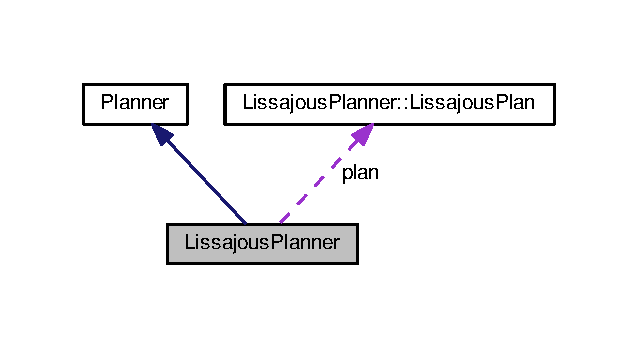
\includegraphics[width=306pt]{classLissajousPlanner__coll__graph}
\end{center}
\end{figure}
\subsection*{Classes}
\begin{DoxyCompactItemize}
\item 
struct \hyperlink{structLissajousPlanner_1_1LissajousPlan}{Lissajous\+Plan}
\end{DoxyCompactItemize}
\subsection*{Public Member Functions}
\begin{DoxyCompactItemize}
\item 
{\bfseries Lissajous\+Planner} (ros\+::\+Node\+Handle \&\hyperlink{classPlanner_a9714d036f444a07ce90be8d135b9a40c}{nh})\hypertarget{classLissajousPlanner_a82095ebb2cd29944a201321377fc78fe}{}\label{classLissajousPlanner_a82095ebb2cd29944a201321377fc78fe}

\item 
void {\bfseries set\+\_\+parameter} (float omegax, float dphi=0.\+0, int ratio=2, float Ax=3.\+0, float Ay=3.\+0)\hypertarget{classLissajousPlanner_aa6e4d941a535dca182aaf8b73b5a0dcd}{}\label{classLissajousPlanner_aa6e4d941a535dca182aaf8b73b5a0dcd}

\item 
void {\bfseries load} ()\hypertarget{classLissajousPlanner_ae7ecff9989a37d29e591bac082b781ac}{}\label{classLissajousPlanner_ae7ecff9989a37d29e591bac082b781ac}

\end{DoxyCompactItemize}
\subsection*{Private Member Functions}
\begin{DoxyCompactItemize}
\item 
tf\+::\+Vector3 {\bfseries get\+\_\+position} (ros\+::\+Duration time)\hypertarget{classLissajousPlanner_aeb9a2e0f3cb8e651518bcd0dcd80bf2f}{}\label{classLissajousPlanner_aeb9a2e0f3cb8e651518bcd0dcd80bf2f}

\item 
tf\+::\+Quaternion {\bfseries get\+\_\+orientation} (ros\+::\+Duration time)\hypertarget{classLissajousPlanner_a07eb5dc306609dd6ae1f91e2738aee95}{}\label{classLissajousPlanner_a07eb5dc306609dd6ae1f91e2738aee95}

\item 
tf\+::\+Vector3 {\bfseries get\+\_\+velocity} (ros\+::\+Duration time)\hypertarget{classLissajousPlanner_a17a85db0fe0f380164297b8365232ab2}{}\label{classLissajousPlanner_a17a85db0fe0f380164297b8365232ab2}

\item 
double {\bfseries get\+\_\+angular\+\_\+velocity} (ros\+::\+Duration time)\hypertarget{classLissajousPlanner_ab7ef88484995f3fd223c8dcbd6f86a8e}{}\label{classLissajousPlanner_ab7ef88484995f3fd223c8dcbd6f86a8e}

\item 
void {\bfseries check\+\_\+period} (ros\+::\+Duration time)\hypertarget{classLissajousPlanner_a9001fcfa7f1d25e4ae7826499b0b2ebc}{}\label{classLissajousPlanner_a9001fcfa7f1d25e4ae7826499b0b2ebc}

\end{DoxyCompactItemize}
\subsection*{Private Attributes}
\begin{DoxyCompactItemize}
\item 
\hyperlink{structLissajousPlanner_1_1LissajousPlan}{Lissajous\+Plan} {\bfseries plan}\hypertarget{classLissajousPlanner_ac3365f9d9d84307b680a94cff01edd9b}{}\label{classLissajousPlanner_ac3365f9d9d84307b680a94cff01edd9b}

\end{DoxyCompactItemize}
\subsection*{Additional Inherited Members}


The documentation for this class was generated from the following files\+:\begin{DoxyCompactItemize}
\item 
simulation\+\_\+env/include/simulation\+\_\+env/planner.\+h\item 
simulation\+\_\+env/src/planner.\+cpp\end{DoxyCompactItemize}

\hypertarget{structController_1_1LyapunovParameter}{}\section{Controller\+:\+:Lyapunov\+Parameter Struct Reference}
\label{structController_1_1LyapunovParameter}\index{Controller\+::\+Lyapunov\+Parameter@{Controller\+::\+Lyapunov\+Parameter}}


Specifies the parameters needed for the lyapunov based control law.  




{\ttfamily \#include $<$controller.\+h$>$}

\subsection*{Public Member Functions}
\begin{DoxyCompactItemize}
\item 
\hyperlink{structController_1_1LyapunovParameter_ae0d081687dfc7637bfbce3fe4cc2d9dd}{Lyapunov\+Parameter} ()\hypertarget{structController_1_1LyapunovParameter_ae0d081687dfc7637bfbce3fe4cc2d9dd}{}\label{structController_1_1LyapunovParameter_ae0d081687dfc7637bfbce3fe4cc2d9dd}

\begin{DoxyCompactList}\small\item\em Construct a new Lyapunov Parameter object with default Parameter. \end{DoxyCompactList}\item 
\hyperlink{structController_1_1LyapunovParameter_acca8d24226201cd98caa44ccd4ddc4ac}{Lyapunov\+Parameter} (float \hyperlink{structController_1_1LyapunovParameter_a4183bf21c97669dc44d4f67cb9a0d26c}{kx}, float \hyperlink{structController_1_1LyapunovParameter_a4cde698202cddb2fb3971fcc0f0804ca}{ky}, float \hyperlink{structController_1_1LyapunovParameter_a4ffd5e85451097367940acc6536d2a4c}{kphi})
\begin{DoxyCompactList}\small\item\em Construct a new Lyapunov Parameter object with given parameters. \end{DoxyCompactList}\item 
\hyperlink{structController_1_1LyapunovParameter_a5c8cfc9a6c9168848ddce0d15f17ec02}{Lyapunov\+Parameter} (std\+::vector$<$ float $>$ param)
\begin{DoxyCompactList}\small\item\em Construct a new Lyapunov Parameter object with given parameters by vector. \end{DoxyCompactList}\end{DoxyCompactItemize}
\subsection*{Public Attributes}
\begin{DoxyCompactItemize}
\item 
float \hyperlink{structController_1_1LyapunovParameter_a4183bf21c97669dc44d4f67cb9a0d26c}{kx}\hypertarget{structController_1_1LyapunovParameter_a4183bf21c97669dc44d4f67cb9a0d26c}{}\label{structController_1_1LyapunovParameter_a4183bf21c97669dc44d4f67cb9a0d26c}

\begin{DoxyCompactList}\small\item\em Control gain in x-\/direction. \end{DoxyCompactList}\item 
float \hyperlink{structController_1_1LyapunovParameter_a4cde698202cddb2fb3971fcc0f0804ca}{ky}\hypertarget{structController_1_1LyapunovParameter_a4cde698202cddb2fb3971fcc0f0804ca}{}\label{structController_1_1LyapunovParameter_a4cde698202cddb2fb3971fcc0f0804ca}

\begin{DoxyCompactList}\small\item\em Control gain in y-\/direction. \end{DoxyCompactList}\item 
float \hyperlink{structController_1_1LyapunovParameter_a4ffd5e85451097367940acc6536d2a4c}{kphi}\hypertarget{structController_1_1LyapunovParameter_a4ffd5e85451097367940acc6536d2a4c}{}\label{structController_1_1LyapunovParameter_a4ffd5e85451097367940acc6536d2a4c}

\begin{DoxyCompactList}\small\item\em Control gain in theta-\/direction. \end{DoxyCompactList}\end{DoxyCompactItemize}


\subsection{Detailed Description}
Specifies the parameters needed for the lyapunov based control law. 

\subsection{Constructor \& Destructor Documentation}
\index{Controller\+::\+Lyapunov\+Parameter@{Controller\+::\+Lyapunov\+Parameter}!Lyapunov\+Parameter@{Lyapunov\+Parameter}}
\index{Lyapunov\+Parameter@{Lyapunov\+Parameter}!Controller\+::\+Lyapunov\+Parameter@{Controller\+::\+Lyapunov\+Parameter}}
\subsubsection[{\texorpdfstring{Lyapunov\+Parameter(float kx, float ky, float kphi)}{LyapunovParameter(float kx, float ky, float kphi)}}]{\setlength{\rightskip}{0pt plus 5cm}Controller\+::\+Lyapunov\+Parameter\+::\+Lyapunov\+Parameter (
\begin{DoxyParamCaption}
\item[{float}]{kx, }
\item[{float}]{ky, }
\item[{float}]{kphi}
\end{DoxyParamCaption}
)\hspace{0.3cm}{\ttfamily [inline]}}\hypertarget{structController_1_1LyapunovParameter_acca8d24226201cd98caa44ccd4ddc4ac}{}\label{structController_1_1LyapunovParameter_acca8d24226201cd98caa44ccd4ddc4ac}


Construct a new Lyapunov Parameter object with given parameters. 


\begin{DoxyParams}{Parameters}
{\em kx} & ///$<$ Gain in kartesian x direction \\
\hline
{\em ky} & ///$<$Gain in kartesian y direction \\
\hline
{\em kphi} & ///$<$Gain in phi direction (around the z axis) \\
\hline
\end{DoxyParams}
\index{Controller\+::\+Lyapunov\+Parameter@{Controller\+::\+Lyapunov\+Parameter}!Lyapunov\+Parameter@{Lyapunov\+Parameter}}
\index{Lyapunov\+Parameter@{Lyapunov\+Parameter}!Controller\+::\+Lyapunov\+Parameter@{Controller\+::\+Lyapunov\+Parameter}}
\subsubsection[{\texorpdfstring{Lyapunov\+Parameter(std\+::vector$<$ float $>$ param)}{LyapunovParameter(std::vector< float > param)}}]{\setlength{\rightskip}{0pt plus 5cm}Controller\+::\+Lyapunov\+Parameter\+::\+Lyapunov\+Parameter (
\begin{DoxyParamCaption}
\item[{std\+::vector$<$ float $>$}]{param}
\end{DoxyParamCaption}
)\hspace{0.3cm}{\ttfamily [inline]}}\hypertarget{structController_1_1LyapunovParameter_a5c8cfc9a6c9168848ddce0d15f17ec02}{}\label{structController_1_1LyapunovParameter_a5c8cfc9a6c9168848ddce0d15f17ec02}


Construct a new Lyapunov Parameter object with given parameters by vector. 


\begin{DoxyParams}{Parameters}
{\em param} & vector that must contain the three object parameters \\
\hline
\end{DoxyParams}


The documentation for this struct was generated from the following file\+:\begin{DoxyCompactItemize}
\item 
controller/include/controller/controller.\+h\end{DoxyCompactItemize}

\hypertarget{classMaster}{}\section{Master Class Reference}
\label{classMaster}\index{Master@{Master}}


Class that implements a master robot for multi robot formation control.  




{\ttfamily \#include $<$master.\+h$>$}



Inheritance diagram for Master\+:\nopagebreak
\begin{figure}[H]
\begin{center}
\leavevmode
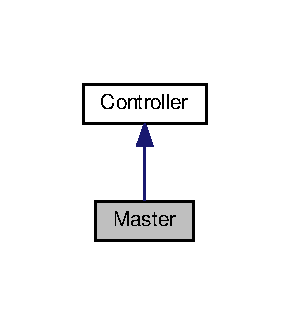
\includegraphics[width=139pt]{classMaster__inherit__graph}
\end{center}
\end{figure}


Collaboration diagram for Master\+:\nopagebreak
\begin{figure}[H]
\begin{center}
\leavevmode
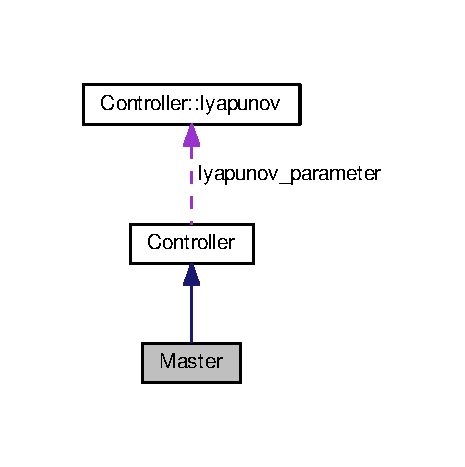
\includegraphics[width=350pt]{classMaster__coll__graph}
\end{center}
\end{figure}
\subsection*{Public Member Functions}
\begin{DoxyCompactItemize}
\item 
\hyperlink{classMaster_ab52840de45f9ce7022c9cf58cfb49398}{Master} (ros\+::\+Node\+Handle \&\hyperlink{classController_a24e3d3c2536f6ed29018bad1fd53dae2}{nh})
\begin{DoxyCompactList}\small\item\em Construct a new \hyperlink{classMaster}{Master} object. \end{DoxyCompactList}\end{DoxyCompactItemize}
\subsection*{Additional Inherited Members}


\subsection{Detailed Description}
Class that implements a master robot for multi robot formation control. 

\subsection{Constructor \& Destructor Documentation}
\index{Master@{Master}!Master@{Master}}
\index{Master@{Master}!Master@{Master}}
\subsubsection[{\texorpdfstring{Master(ros\+::\+Node\+Handle \&nh)}{Master(ros::NodeHandle &nh)}}]{\setlength{\rightskip}{0pt plus 5cm}Master\+::\+Master (
\begin{DoxyParamCaption}
\item[{ros\+::\+Node\+Handle \&}]{nh}
\end{DoxyParamCaption}
)}\hypertarget{classMaster_ab52840de45f9ce7022c9cf58cfb49398}{}\label{classMaster_ab52840de45f9ce7022c9cf58cfb49398}


Construct a new \hyperlink{classMaster}{Master} object. 


\begin{DoxyParams}{Parameters}
{\em nh} & Nodehandle \\
\hline
\end{DoxyParams}


The documentation for this class was generated from the following files\+:\begin{DoxyCompactItemize}
\item 
controller/include/controller/master.\+h\item 
controller/src/master.\+cpp\end{DoxyCompactItemize}

\hypertarget{classPlanner}{}\section{Planner Class Reference}
\label{classPlanner}\index{Planner@{Planner}}


Inheritance diagram for Planner\+:\nopagebreak
\begin{figure}[H]
\begin{center}
\leavevmode
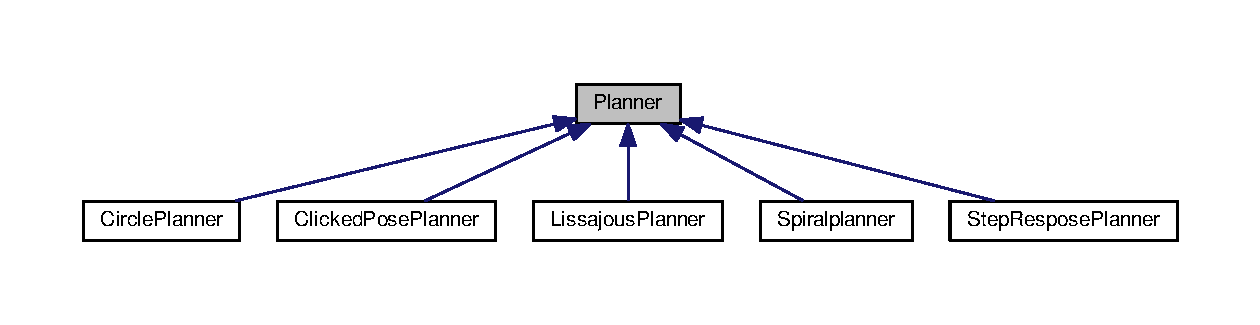
\includegraphics[width=264pt]{classPlanner__inherit__graph}
\end{center}
\end{figure}
\subsection*{Public Member Functions}
\begin{DoxyCompactItemize}
\item 
{\bfseries Planner} (ros\+::\+Node\+Handle \&\hyperlink{classPlanner_a9714d036f444a07ce90be8d135b9a40c}{nh})\hypertarget{classPlanner_a32475baddd401921adb1aab3ab842210}{}\label{classPlanner_a32475baddd401921adb1aab3ab842210}

\item 
void {\bfseries start} ()\hypertarget{classPlanner_a6c1c8d67d0cac41f738b413d1833c007}{}\label{classPlanner_a6c1c8d67d0cac41f738b413d1833c007}

\item 
void {\bfseries stop} ()\hypertarget{classPlanner_a3d0a3d404d39f59bfc21f275b0da408a}{}\label{classPlanner_a3d0a3d404d39f59bfc21f275b0da408a}

\item 
void {\bfseries pause} ()\hypertarget{classPlanner_a400f2aefad591e55a62e0fb13cb02521}{}\label{classPlanner_a400f2aefad591e55a62e0fb13cb02521}

\item 
void {\bfseries set\+\_\+start\+\_\+pose} (tf\+::\+Pose pose)\hypertarget{classPlanner_acaf55e0e250d6f3ba14bfcf3c4f06ffb}{}\label{classPlanner_acaf55e0e250d6f3ba14bfcf3c4f06ffb}

\item 
virtual void {\bfseries load} ()=0\hypertarget{classPlanner_af10d045ffe58c7d2149156567dc8b10a}{}\label{classPlanner_af10d045ffe58c7d2149156567dc8b10a}

\end{DoxyCompactItemize}
\subsection*{Protected Attributes}
\begin{DoxyCompactItemize}
\item 
int {\bfseries iterations\+\_\+counter}\hypertarget{classPlanner_a99b577203757a2466e8a3424c28d3449}{}\label{classPlanner_a99b577203757a2466e8a3424c28d3449}

\item 
ros\+::\+Node\+Handle \hyperlink{classPlanner_a9714d036f444a07ce90be8d135b9a40c}{nh}\hypertarget{classPlanner_a9714d036f444a07ce90be8d135b9a40c}{}\label{classPlanner_a9714d036f444a07ce90be8d135b9a40c}

\begin{DoxyCompactList}\small\item\em Counter for the iterations of periodic planner functions. \end{DoxyCompactList}\end{DoxyCompactItemize}
\subsection*{Private Member Functions}
\begin{DoxyCompactItemize}
\item 
void {\bfseries plan} (const ros\+::\+Timer\+Event \&events)\hypertarget{classPlanner_a6ccd3cb4a24886ddeff615e665f2fbbd}{}\label{classPlanner_a6ccd3cb4a24886ddeff615e665f2fbbd}

\item 
void {\bfseries publish} ()\hypertarget{classPlanner_aa8937e0a808cebc224393438941515e4}{}\label{classPlanner_aa8937e0a808cebc224393438941515e4}

\item 
tf\+::\+Transform \hyperlink{classPlanner_a311803ff0901b953c4ff9db7a3f5bb01}{get\+\_\+transform} (tf\+::\+Pose pose)
\item 
void \hyperlink{classPlanner_a0ce8028259452e2e17ed07bbb0c8463a}{transform\+\_\+values} (tf\+::\+Transform trafo)
\item 
bool \hyperlink{classPlanner_aef1abb6588a8fb7953183bc5f3479857}{srv\+\_\+start} (std\+\_\+srvs\+::\+Set\+Bool\+::\+Request \&req, std\+\_\+srvs\+::\+Set\+Bool\+::\+Response \&res)
\item 
bool \hyperlink{classPlanner_ac98453a1cd02d1d77055900f4fc4741f}{srv\+\_\+stop} (std\+\_\+srvs\+::\+Set\+Bool\+::\+Request \&req, std\+\_\+srvs\+::\+Set\+Bool\+::\+Response \&res)
\item 
virtual tf\+::\+Vector3 {\bfseries get\+\_\+position} (ros\+::\+Duration time)=0\hypertarget{classPlanner_ab388545a3fd2f37f70403d8484473a12}{}\label{classPlanner_ab388545a3fd2f37f70403d8484473a12}

\item 
virtual tf\+::\+Quaternion {\bfseries get\+\_\+orientation} (ros\+::\+Duration time)=0\hypertarget{classPlanner_a161fc00d031fd65914dae8f4b2edeffb}{}\label{classPlanner_a161fc00d031fd65914dae8f4b2edeffb}

\item 
virtual tf\+::\+Vector3 {\bfseries get\+\_\+velocity} (ros\+::\+Duration time)=0\hypertarget{classPlanner_a02af8b9ab29a19bd82c1cc35afcf2cc5}{}\label{classPlanner_a02af8b9ab29a19bd82c1cc35afcf2cc5}

\item 
virtual double {\bfseries get\+\_\+angular\+\_\+velocity} (ros\+::\+Duration time)=0\hypertarget{classPlanner_ab5c6ec661acf83b1f095ba404dc4c958}{}\label{classPlanner_ab5c6ec661acf83b1f095ba404dc4c958}

\item 
virtual void {\bfseries check\+\_\+period} (ros\+::\+Duration time)=0\hypertarget{classPlanner_a1bc7f9ca05b5de8aa4c9ccda126c2be2}{}\label{classPlanner_a1bc7f9ca05b5de8aa4c9ccda126c2be2}

\end{DoxyCompactItemize}
\subsection*{Private Attributes}
\begin{DoxyCompactItemize}
\item 
ros\+::\+Timer {\bfseries tim\+\_\+sampling}\hypertarget{classPlanner_a8dd2352bf15aef91d49337d95dfe6b04}{}\label{classPlanner_a8dd2352bf15aef91d49337d95dfe6b04}

\item 
ros\+::\+Publisher {\bfseries pub\+\_\+current\+\_\+odometry}\hypertarget{classPlanner_a1eea64fbf5b532bedd2f5a20eaedb4d8}{}\label{classPlanner_a1eea64fbf5b532bedd2f5a20eaedb4d8}

\item 
ros\+::\+Service\+Server {\bfseries set\+\_\+start\+\_\+service}\hypertarget{classPlanner_ad3cb4222b988ec69a5b89e1c67b119cd}{}\label{classPlanner_ad3cb4222b988ec69a5b89e1c67b119cd}

\item 
ros\+::\+Service\+Server {\bfseries set\+\_\+stop\+\_\+service}\hypertarget{classPlanner_a9211a5e71956ef94e1306adcabb2e51d}{}\label{classPlanner_a9211a5e71956ef94e1306adcabb2e51d}

\item 
bool {\bfseries is\+\_\+planning}\hypertarget{classPlanner_afcb5f703c4d2a54bb8c8f8360864b763}{}\label{classPlanner_afcb5f703c4d2a54bb8c8f8360864b763}

\item 
bool {\bfseries is\+\_\+paused}\hypertarget{classPlanner_a247ba912994c9035473b9ee037aac307}{}\label{classPlanner_a247ba912994c9035473b9ee037aac307}

\item 
int {\bfseries iterations}\hypertarget{classPlanner_a19220ea8cd70f4f3bfa3e35e1250ed00}{}\label{classPlanner_a19220ea8cd70f4f3bfa3e35e1250ed00}

\item 
std\+::string {\bfseries frame\+\_\+name}\hypertarget{classPlanner_a1578a9b87a63d6a806ab46a863ec55cb}{}\label{classPlanner_a1578a9b87a63d6a806ab46a863ec55cb}

\item 
ros\+::\+Duration {\bfseries paused}\hypertarget{classPlanner_a0e99faac21bce026cb9b0b576b734c71}{}\label{classPlanner_a0e99faac21bce026cb9b0b576b734c71}

\item 
ros\+::\+Time {\bfseries start\+\_\+time}\hypertarget{classPlanner_ade39963b5d3f74b75feed62ab669979e}{}\label{classPlanner_ade39963b5d3f74b75feed62ab669979e}

\item 
tf\+::\+Pose {\bfseries start\+\_\+pose}\hypertarget{classPlanner_af8043c3dfe8d863cec156f6b5abddd76}{}\label{classPlanner_af8043c3dfe8d863cec156f6b5abddd76}

\item 
tf\+::\+Vector3 {\bfseries planned\+\_\+vel}\hypertarget{classPlanner_a3d271654bd61b688e1db4f942722dd53}{}\label{classPlanner_a3d271654bd61b688e1db4f942722dd53}

\item 
tf\+::\+Vector3 {\bfseries vel}\hypertarget{classPlanner_aae4477f491ca6ba2e7f9ec2f0ca297c6}{}\label{classPlanner_aae4477f491ca6ba2e7f9ec2f0ca297c6}

\item 
tf\+::\+Vector3 {\bfseries pos}\hypertarget{classPlanner_a0f68f1ba4044c5a451e9352aed57ab9f}{}\label{classPlanner_a0f68f1ba4044c5a451e9352aed57ab9f}

\item 
tf\+::\+Quaternion {\bfseries orientation}\hypertarget{classPlanner_a3ce130c29c044931c6e8e7eeffd24c25}{}\label{classPlanner_a3ce130c29c044931c6e8e7eeffd24c25}

\item 
double {\bfseries ang\+\_\+vel}\hypertarget{classPlanner_a026af8deca2879d9f16b9eeddd003d88}{}\label{classPlanner_a026af8deca2879d9f16b9eeddd003d88}

\item 
tf\+::\+Transform {\bfseries start\+\_\+reference}\hypertarget{classPlanner_aae0304ebd1813766f1437b80d5195e90}{}\label{classPlanner_aae0304ebd1813766f1437b80d5195e90}

\end{DoxyCompactItemize}


\subsection{Member Function Documentation}
\index{Planner@{Planner}!get\+\_\+transform@{get\+\_\+transform}}
\index{get\+\_\+transform@{get\+\_\+transform}!Planner@{Planner}}
\subsubsection[{\texorpdfstring{get\+\_\+transform(tf\+::\+Pose pose)}{get_transform(tf::Pose pose)}}]{\setlength{\rightskip}{0pt plus 5cm}tf\+::\+Transform Planner\+::get\+\_\+transform (
\begin{DoxyParamCaption}
\item[{tf\+::\+Pose}]{pose}
\end{DoxyParamCaption}
)\hspace{0.3cm}{\ttfamily [private]}}\hypertarget{classPlanner_a311803ff0901b953c4ff9db7a3f5bb01}{}\label{classPlanner_a311803ff0901b953c4ff9db7a3f5bb01}
Gets the transformation form the given pose to the pose at timestamp zero 
\begin{DoxyParams}{Parameters}
{\em pose} & \+: Pose from wich the planner should start \\
\hline
\end{DoxyParams}
\index{Planner@{Planner}!srv\+\_\+start@{srv\+\_\+start}}
\index{srv\+\_\+start@{srv\+\_\+start}!Planner@{Planner}}
\subsubsection[{\texorpdfstring{srv\+\_\+start(std\+\_\+srvs\+::\+Set\+Bool\+::\+Request \&req, std\+\_\+srvs\+::\+Set\+Bool\+::\+Response \&res)}{srv_start(std_srvs::SetBool::Request &req, std_srvs::SetBool::Response &res)}}]{\setlength{\rightskip}{0pt plus 5cm}bool Planner\+::srv\+\_\+start (
\begin{DoxyParamCaption}
\item[{std\+\_\+srvs\+::\+Set\+Bool\+::\+Request \&}]{req, }
\item[{std\+\_\+srvs\+::\+Set\+Bool\+::\+Response \&}]{res}
\end{DoxyParamCaption}
)\hspace{0.3cm}{\ttfamily [private]}}\hypertarget{classPlanner_aef1abb6588a8fb7953183bc5f3479857}{}\label{classPlanner_aef1abb6588a8fb7953183bc5f3479857}
service procedure for satrting the planner 
\begin{DoxyParams}{Parameters}
{\em req} & \+: Reqest the service is getting \\
\hline
{\em res} & \+: Response the service is sending \\
\hline
\end{DoxyParams}
\index{Planner@{Planner}!srv\+\_\+stop@{srv\+\_\+stop}}
\index{srv\+\_\+stop@{srv\+\_\+stop}!Planner@{Planner}}
\subsubsection[{\texorpdfstring{srv\+\_\+stop(std\+\_\+srvs\+::\+Set\+Bool\+::\+Request \&req, std\+\_\+srvs\+::\+Set\+Bool\+::\+Response \&res)}{srv_stop(std_srvs::SetBool::Request &req, std_srvs::SetBool::Response &res)}}]{\setlength{\rightskip}{0pt plus 5cm}bool Planner\+::srv\+\_\+stop (
\begin{DoxyParamCaption}
\item[{std\+\_\+srvs\+::\+Set\+Bool\+::\+Request \&}]{req, }
\item[{std\+\_\+srvs\+::\+Set\+Bool\+::\+Response \&}]{res}
\end{DoxyParamCaption}
)\hspace{0.3cm}{\ttfamily [private]}}\hypertarget{classPlanner_ac98453a1cd02d1d77055900f4fc4741f}{}\label{classPlanner_ac98453a1cd02d1d77055900f4fc4741f}
service procedure for stopping the planner 
\begin{DoxyParams}{Parameters}
{\em req} & \+: Reqest the service is getting \\
\hline
{\em res} & \+: Response the service is sending \\
\hline
\end{DoxyParams}
\index{Planner@{Planner}!transform\+\_\+values@{transform\+\_\+values}}
\index{transform\+\_\+values@{transform\+\_\+values}!Planner@{Planner}}
\subsubsection[{\texorpdfstring{transform\+\_\+values(tf\+::\+Transform trafo)}{transform_values(tf::Transform trafo)}}]{\setlength{\rightskip}{0pt plus 5cm}void Planner\+::transform\+\_\+values (
\begin{DoxyParamCaption}
\item[{tf\+::\+Transform}]{trafo}
\end{DoxyParamCaption}
)\hspace{0.3cm}{\ttfamily [private]}}\hypertarget{classPlanner_a0ce8028259452e2e17ed07bbb0c8463a}{}\label{classPlanner_a0ce8028259452e2e17ed07bbb0c8463a}
Transforming all values that are not rotation or translation invariant 
\begin{DoxyParams}{Parameters}
{\em trafo} & \+: The Transformation applied to all values \\
\hline
\end{DoxyParams}


The documentation for this class was generated from the following files\+:\begin{DoxyCompactItemize}
\item 
simulation\+\_\+env/include/simulation\+\_\+env/planner.\+h\item 
simulation\+\_\+env/src/planner.\+cpp\end{DoxyCompactItemize}

\hypertarget{classSlave}{}\section{Slave Class Reference}
\label{classSlave}\index{Slave@{Slave}}


Inheritance diagram for Slave\+:\nopagebreak
\begin{figure}[H]
\begin{center}
\leavevmode
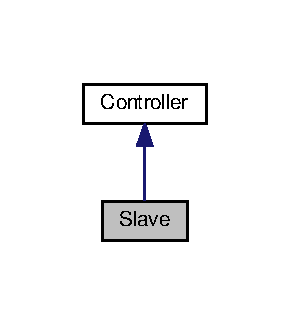
\includegraphics[width=139pt]{classSlave__inherit__graph}
\end{center}
\end{figure}


Collaboration diagram for Slave\+:\nopagebreak
\begin{figure}[H]
\begin{center}
\leavevmode
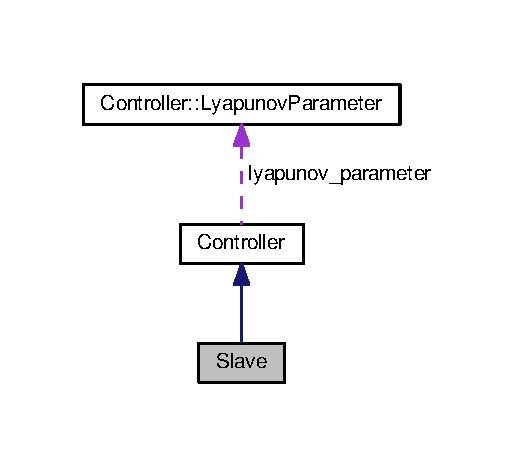
\includegraphics[width=223pt]{classSlave__coll__graph}
\end{center}
\end{figure}
\subsection*{Public Member Functions}
\begin{DoxyCompactItemize}
\item 
{\bfseries Slave} (ros\+::\+Node\+Handle \&\hyperlink{classController_a24e3d3c2536f6ed29018bad1fd53dae2}{nh})\hypertarget{classSlave_a855a824b462dd05eddaa8d53b27faea4}{}\label{classSlave_a855a824b462dd05eddaa8d53b27faea4}

\item 
void \hyperlink{classSlave_a9b5d1d499c7bd05d5260fbe5b8afbbb5}{scope} ()\hypertarget{classSlave_a9b5d1d499c7bd05d5260fbe5b8afbbb5}{}\label{classSlave_a9b5d1d499c7bd05d5260fbe5b8afbbb5}

\begin{DoxyCompactList}\small\item\em A Scope within the execute function. Repeating calculation in inheriting classes are implemented here. \end{DoxyCompactList}\end{DoxyCompactItemize}
\subsection*{Private Member Functions}
\begin{DoxyCompactItemize}
\item 
void \hyperlink{classSlave_a2a38a730d6ac93fcced035a7d764612d}{optimal\+\_\+control} ()
\item 
void \hyperlink{classSlave_a09394d0f823a06e04f6259ee490bc867}{target\+\_\+state\+\_\+callback} (geometry\+\_\+msgs\+::\+Pose\+Stamped msg)\hypertarget{classSlave_a09394d0f823a06e04f6259ee490bc867}{}\label{classSlave_a09394d0f823a06e04f6259ee490bc867}

\begin{DoxyCompactList}\small\item\em Callback for input target state message. Is executed everytima a target state input is incoming. Writes data to target\+\_\+pose state. \end{DoxyCompactList}\item 
void \hyperlink{classSlave_a2227f30ab058b623de7f6a940d079c90}{target\+\_\+velocities\+\_\+callback} (geometry\+\_\+msgs\+::\+Twist msg)\hypertarget{classSlave_a2227f30ab058b623de7f6a940d079c90}{}\label{classSlave_a2227f30ab058b623de7f6a940d079c90}

\begin{DoxyCompactList}\small\item\em Callback for input velocitiy message. Is executed everytime a velocitiy input is incoming. Writes data to input state. \end{DoxyCompactList}\item 
void \hyperlink{classSlave_a0d732637d1c0d06c214112a381ead6be}{target\+\_\+odometry\+\_\+callback} (nav\+\_\+msgs\+::\+Odometry msg)\hypertarget{classSlave_a0d732637d1c0d06c214112a381ead6be}{}\label{classSlave_a0d732637d1c0d06c214112a381ead6be}

\begin{DoxyCompactList}\small\item\em Callback for input target odometry message. Is executed everytima a target odometry input is incoming. Writes data to target\+\_\+pose state and target\+\_\+vel. \end{DoxyCompactList}\end{DoxyCompactItemize}
\subsection*{Private Attributes}
\begin{DoxyCompactItemize}
\item 
ros\+::\+Subscriber {\bfseries master\+\_\+odom}\hypertarget{classSlave_ae16b74032864ebb31211f992d37a73ab}{}\label{classSlave_ae16b74032864ebb31211f992d37a73ab}

\item 
tf\+::\+Pose {\bfseries master\+\_\+pose}\hypertarget{classSlave_ab6effa214fce2263784c296ecba8d3e0}{}\label{classSlave_ab6effa214fce2263784c296ecba8d3e0}

\end{DoxyCompactItemize}
\subsection*{Additional Inherited Members}


\subsection{Member Function Documentation}
\index{Slave@{Slave}!optimal\+\_\+control@{optimal\+\_\+control}}
\index{optimal\+\_\+control@{optimal\+\_\+control}!Slave@{Slave}}
\subsubsection[{\texorpdfstring{optimal\+\_\+control()}{optimal_control()}}]{\setlength{\rightskip}{0pt plus 5cm}void Slave\+::optimal\+\_\+control (
\begin{DoxyParamCaption}
{}
\end{DoxyParamCaption}
)\hspace{0.3cm}{\ttfamily [private]}}\hypertarget{classSlave_a2a38a730d6ac93fcced035a7d764612d}{}\label{classSlave_a2a38a730d6ac93fcced035a7d764612d}
This implements a least sqaures determination of control vector \mbox{[}v,omega\mbox{]} \mbox{[}control.\+v control.\+omega\mbox{]} from the given cartesian velocity state d/dt\mbox{[}x,y,phi\mbox{]} (cart\+\_\+vel) 

The documentation for this class was generated from the following files\+:\begin{DoxyCompactItemize}
\item 
controller/include/controller/slave.\+h\item 
controller/src/slave.\+cpp\end{DoxyCompactItemize}

%--- End generated contents ---

% Index
\backmatter
\newpage
\phantomsection
\clearemptydoublepage
\addcontentsline{toc}{chapter}{Index}
\printindex

\end{document}
